\documentclass[12pt,a4paper]{report}

% --- Paquetes esenciales para idioma, codificación y tipografía ---
\usepackage[utf8]{inputenc}
\usepackage[spanish,es-tabla,es-noquoting]{babel}
\usepackage{microtype} % Mejora el espaciado y la justificación del texto
\usepackage[autostyle=true, spanish=spanish]{csquotes}
\setquotestyle{english} % Forces standard " " quotes

% --- Paquetes para matemáticas, imágenes y tablas ---
\usepackage{amsmath, amsfonts, amssymb}
\usepackage{graphicx}
\usepackage{float}
\usepackage{booktabs} % Para crear tablas de aspecto profesional
\usepackage{tikz}
\usepackage{tikz-3dplot}
\usetikzlibrary{3d, calc}
\usepackage{multirow}
%\usepackage{parskip}

% ── Bibliografía IEEE con BibTeX ──────────────────────────────────────────────
% Requiere el paquete IEEEtran.bst (incluido en la mayoría de distribuciones TeX)
\bibliographystyle{IEEEtran}

% --- Configuración de página y márgenes ---
\usepackage{geometry}
\geometry{
	a4paper,
	left=2.5cm,
	right=2.5cm,
	top=3cm,
	bottom=3cm,
}


% --- Configuración de encabezados y pies de página ---
\usepackage{fancyhdr}
\pagestyle{fancy}
\fancyhf{} % Limpia los encabezados y pies por defecto
\fancyhead[L]{\nouppercase{\leftmark}} % Nombre del capítulo a la izquierda
\fancyhead[R]{\thepage} % Número de página a la derecha
\renewcommand{\headrulewidth}{0.4pt} % Línea separadora en el encabezado

% --- Configuración de listings para código Python ---
\usepackage{listings}
\usepackage{longtable}
\usepackage[table]{xcolor} % El parámetro table es necesario para colorear celdas
% Definición de colores personalizados para el código
\definecolor{codegreen}{rgb}{0,0.6,0}
\definecolor{codegray}{rgb}{0.5,0.5,0.5}
\definecolor{codepurple}{rgb}{0.58,0,0.82}
\definecolor{backcolour}{rgb}{0.96,0.96,0.94}

\lstset{
	language=Python,
	backgroundcolor=\color{backcolour},
	basicstyle=\ttfamily\footnotesize,
	keywordstyle=\color{blue}\bfseries,
	stringstyle=\color{codepurple},
	commentstyle=\color{codegreen},
	numberstyle=\tiny\color{codegray},
	numbers=left,
	stepnumber=1,
	numbersep=10pt,
	breaklines=true,
	frame=single,
	rulecolor=\color{black!30},
	showstringspaces=false,
	captionpos=b,
	tabsize=4
}

% --- Paquete para hipervínculos (debe ser el último paquete importado) ---
\usepackage{hyperref}
\hypersetup{
	colorlinks=true,
	linkcolor=blue!60!black,
	filecolor=magenta,
	urlcolor=cyan,
	citecolor=green!60!black,
	pdftitle={Análisis de la Red de Dependencias de Python},
	pdfauthor={Bogurad Barañski Barañska, Jorge Bengoa Pinedo}
}

\begin{document}
	
	% ==========================================
	% PORTADA PROFESIONAL
	% ==========================================
	\begin{titlepage}
		\centering
		\vspace*{2cm}
		
		% Puedes añadir el logo de tu universidad aquí si lo deseas
		% \includegraphics[width=0.3\textwidth]{logo.png}\par\vspace{1cm}
		
		{\scshape\LARGE Universidad Politécnica de Madrid \par}
		\vspace{1cm}
		{\scshape\Large Trabajo Final de MINT\par}
		\vspace{1.5cm}
		
		\rule{\textwidth}{0.4pt}\par
		\vspace{0.4cm}
		{\huge\bfseries Análisis de la Red de Dependencias de Python\par}
		\vspace{0.4cm}
		\rule{\textwidth}{0.4pt}\par
		\vspace{2cm}
		
		{\Large\itshape
			Bogurad Barañski Barañska \\
			Jorge Bengoa Pinedo\par
		}
		\vspace{2cm}
		
		\vfill
		% Supervisado por:\par
		% \vspace{0.2cm}
		% {\large Dr. Nombre del Profesor\par}
		
		\vspace{2cm}
		{\large \today\par}
	\end{titlepage}
	
	% ==========================================
	% ÍNDICES
	% ==========================================
	\pagenumbering{roman} % Números romanos para el índice
	\tableofcontents
	\newpage
	
	% Descomentar si vas a tener figuras o tablas en el reporte
	% \listoffigures
	% \newpage
	% \listoftables
	% \newpage
	
	\pagenumbering{arabic} % Números arábigos para el contenido
	
	% ==========================================
	% CAPÍTULO 1: INTRODUCCIÓN
	% ==========================================
	\chapter{Introducción}
	
	\section{Descripción de la Red Propuesta}
	En este trabajo se va a analizar la red de dependencias del ecosistema de paquetes de Python. La red consiste en un grafo dirigido donde los nodos representan paquetes de software y las aristas dirigidas representan las dependencias entre ellos (un paquete requiere de otro para su instalación o funcionamiento). 
	
	\section{Construcción de la Red}
	La red se construye mediante un proceso de extracción de datos automatizado (\textit{web scraping}) haciendo uso de la API pública en formato JSON de PyPI mediante el script \texttt{create\_network.py}. Se parte de una lista de 10 paquetes semilla representativos de distintas áreas, y se aplica un algoritmo de búsqueda recursivo. Por cada paquete, se extraen sus dependencias directas de forma asíncrona, añadiéndolas a la cola de procesamiento hasta alcanzar el volumen deseado para el estudio. 
	
	\section{Herramientas Utilizadas}
	En esta sección se detallan las características del Hardware empleado junto con las versiones del Softwarw utilizado.
	
	\subsection{Características del Equipo}
	Se ha utilizado un portátil con las siguientes características:
	\begin{itemize}
		\item \textbf{Sistema Operativo:} Microsoft Windows 11 Home (Versión 10.0.26200)
		\item \textbf{Procesador (CPU):} Intel(R) Core(TM) i7-8750H CPU @ 2.20GHz
		\item \textbf{Memoria RAM:} 16 GB
	\end{itemize}
	
	\subsection{Software empleado}
	Como lenguaje de programación se ha utilizado \textbf{Python} en la versión \textbf{3.13.7}. Las librerías y dependencias principales utilizadas son:
	\begin{itemize}
		\item \texttt{networkx==3.6.1}: Para la construcción de la red y procesado preliminar.
		\item \texttt{igraph==1.0.0}: Para el cálculo eficiente en grafos.
		\item \texttt{pandas==2.3.2}: Para la estructuración y manejo de los datos.
		\item \texttt{aiohttp==3.13.3}: Para la ejecución segura de peticiones web asíncronas a la API de PyPI durante la fase de recolección de datos.
		\item \texttt{vispy==0.16.1}: Para el renderizado interactivo del motor de físicas del grafo, haciendo uso de la aceleración gráfica (GPU).
		\item \texttt{numpy==2.3.3}: Para el manejo eficiente de operaciones matriciales y vectorización de las fuerzas en el motor de renderizado.
		\item \texttt{matplotlib==3.10.7}: Para la generación visual de tablas y gráficos estáticos de soporte durante el análisis.
	\end{itemize}

	
	\section{Objetivos del Estudio}
	Los objetivos principales de este análisis son:
	\begin{enumerate}
		\item Obtener una visión macroscópica de la estructura del ecosistema de desarrollo de Python.
		\item Identificar los paquetes \textit{hub} o nodos centrales que actúan como dependencias críticas transversales para la mayoría de los proyectos.
		\item Detectar comunidades o clústeres de paquetes que tienden a utilizarse conjuntamente dentro de dominios de desarrollo específicos.
	\end{enumerate}
	
	\chapter{Análisis de la red}
	\section{Descripción de la red}
	En la red de dependencias de Python estudiada los nodos representan las librerías mientras que las aristas son las dependencias. De esta forma, un nodo $A$ apuntará a otro nodo $B$ si depende de él $A \rightarrow B$. Si $B$, además, depende de $C$ pero $A$ lo hace a través de $B$, no existe el enlace entre $A$ y $C$. Las figuras \ref{fig:totalall} y \ref{fig:totalcenter} ilustran la red completa y un zoom de su centro, respectivamente.\\
	
	\begin{figure}[H]
		\centering
		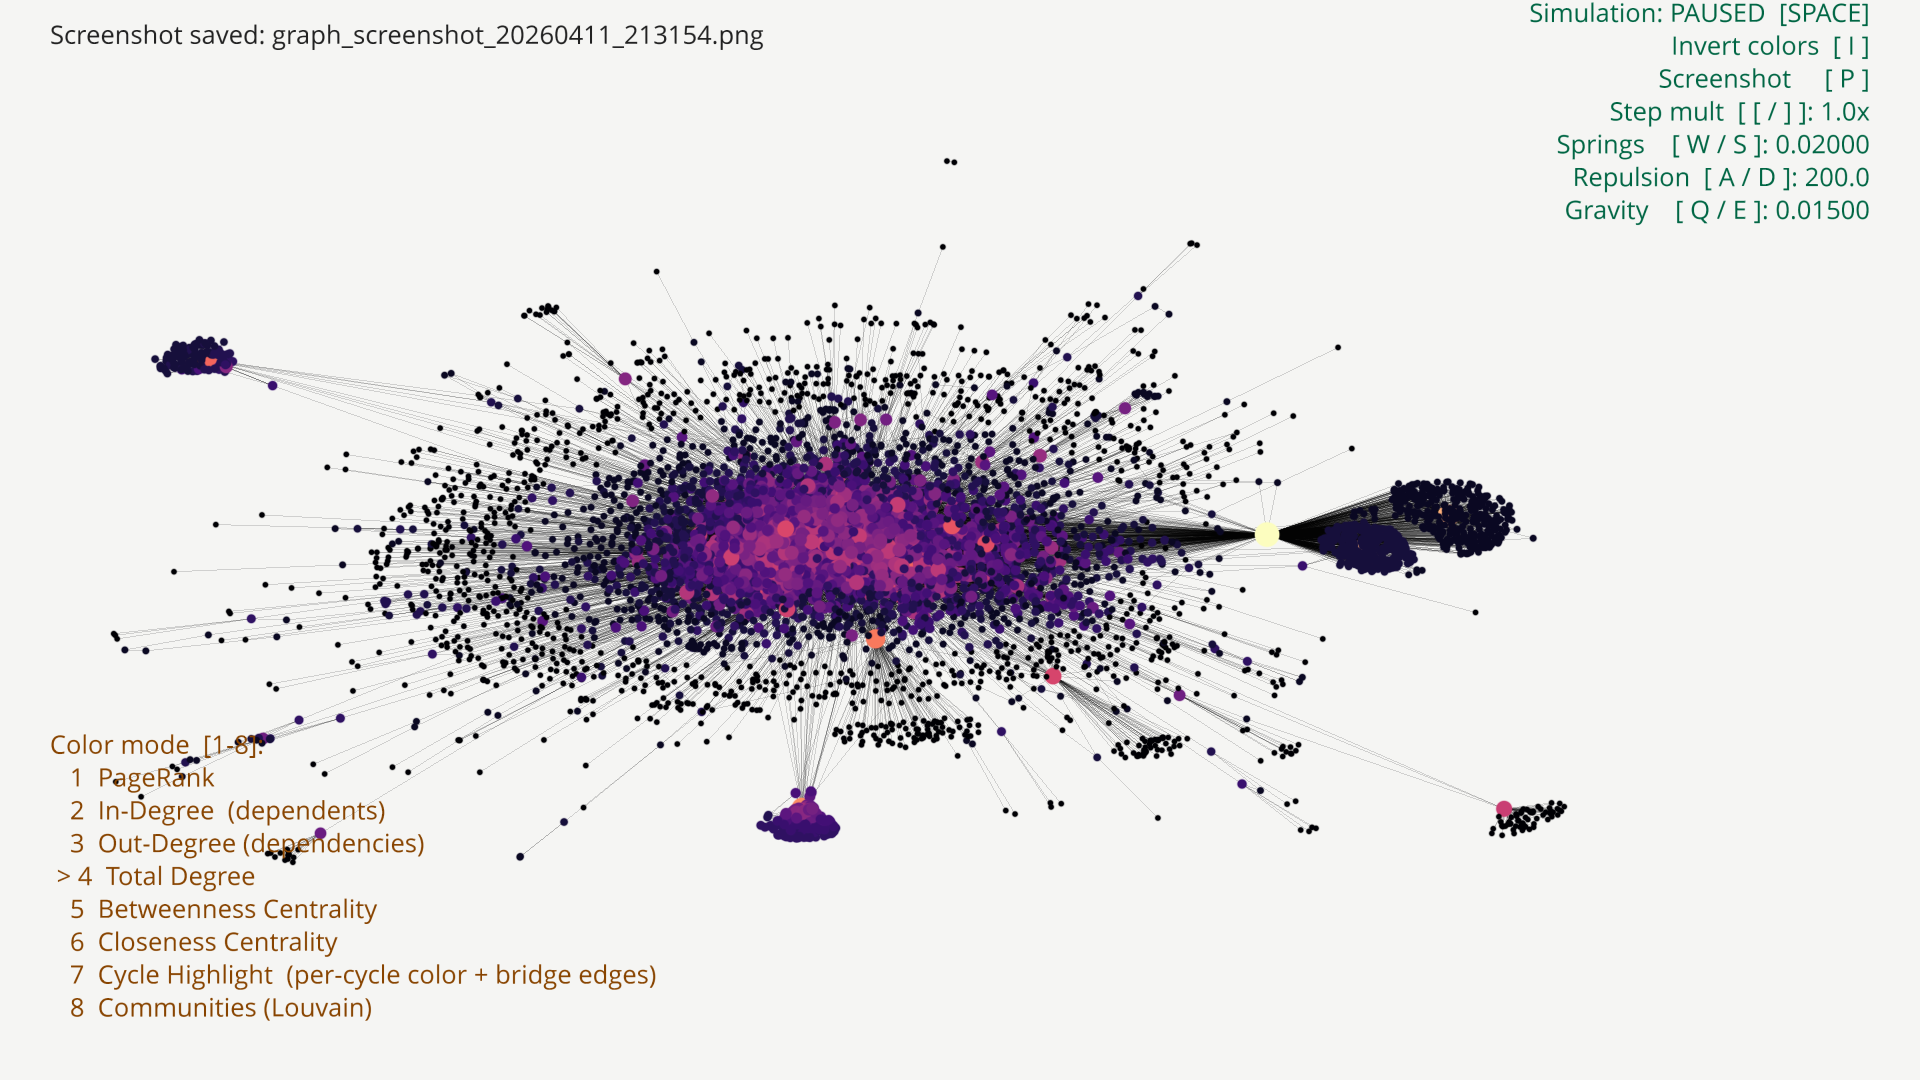
\includegraphics[width=1\linewidth]{Imagenes/TOTAL_ALL}
		\caption{Representación del grado total de los nodos de la red explotada en su totalidad.}
		\label{fig:totalall}
	\end{figure}
	
	
	\begin{figure}[H]
		\centering
		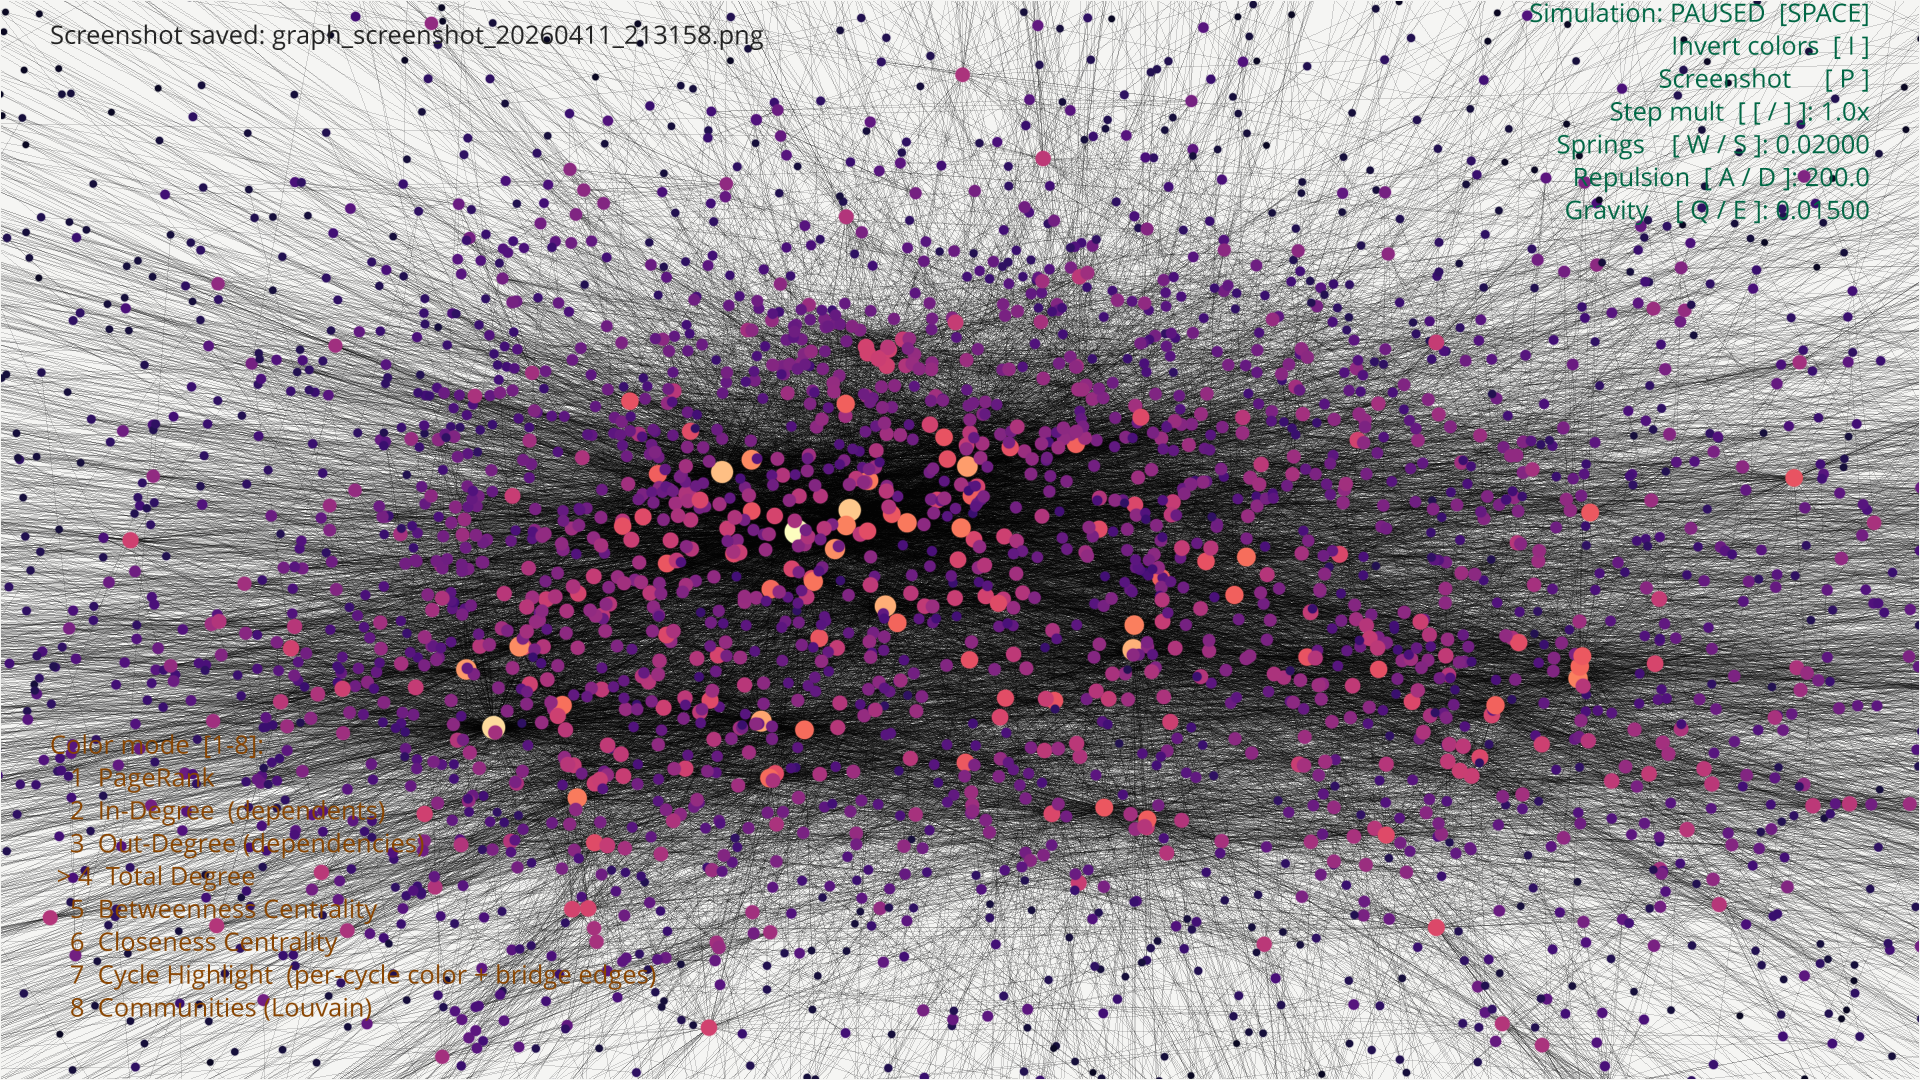
\includegraphics[width=1\linewidth]{Imagenes/TOTAL_CENTER}
		\caption{Representación del grado total de los nodos de la red explotada con zoom a la agrupación central.}
		\label{fig:totalcenter}
	\end{figure}
	
	La red analizada es dirigida con \(6765\) nodos y \(36054\) aristas. Visualmente se representa el grado de entrada de los nodos (figuras \ref{fig:inall} y \ref{fig:incenter}) y de salida (figuras \ref{fig:outall} y \ref{fig:outcenter}). La densidad es muy baja, \(0.000788\), lo que encaja con la idea de que los desarrolladores incluyen un número pequeño de dependencias en sus programas respecto del total de la red. \\
	
	El coeficiente de clustering medio es de 0.3170. Dado que es un valor muy superior a la densidad de la red se puede decir que el clustering es alto. La propiedad de mundo pequeño se ve perjudicada, pues las dependencias de un paquete tienen mayor probabilidad de a depender entre sí. Posiblemente, las distancias entre distintos puntos de la red tiendan a ser grandes. Además, el coeficiente global de clustering es 0.03584. Esto sugiere que los paquetes forman grupos aislados que se conectan a través de hubs con muchas conexiones. Sin embargo, los nodos de un grupo no están conectados directamente a los de otro grupo. \\
	
	El comportamiento descrito tiene sentido desde la perspectiva del desarrollo de paquetes. Los hubs son librerías conocidas que dan acceso a \textit{frameworks} enteros. Los desarrolladores incluyen los hubs en sus programas, no cada una de las dependencias menos conocidas. Los paquetes dentro de un mismo \textit{framework} tienen un objetivo en común, por lo que interactúan entre sí para conseguirlo. Adicionalmente, podrán interactuar con hubs a otros \textit{frameworks}, pero no directamente con cada una de las librerías que contienen.
	
	\begin{figure}[H]
		\centering
		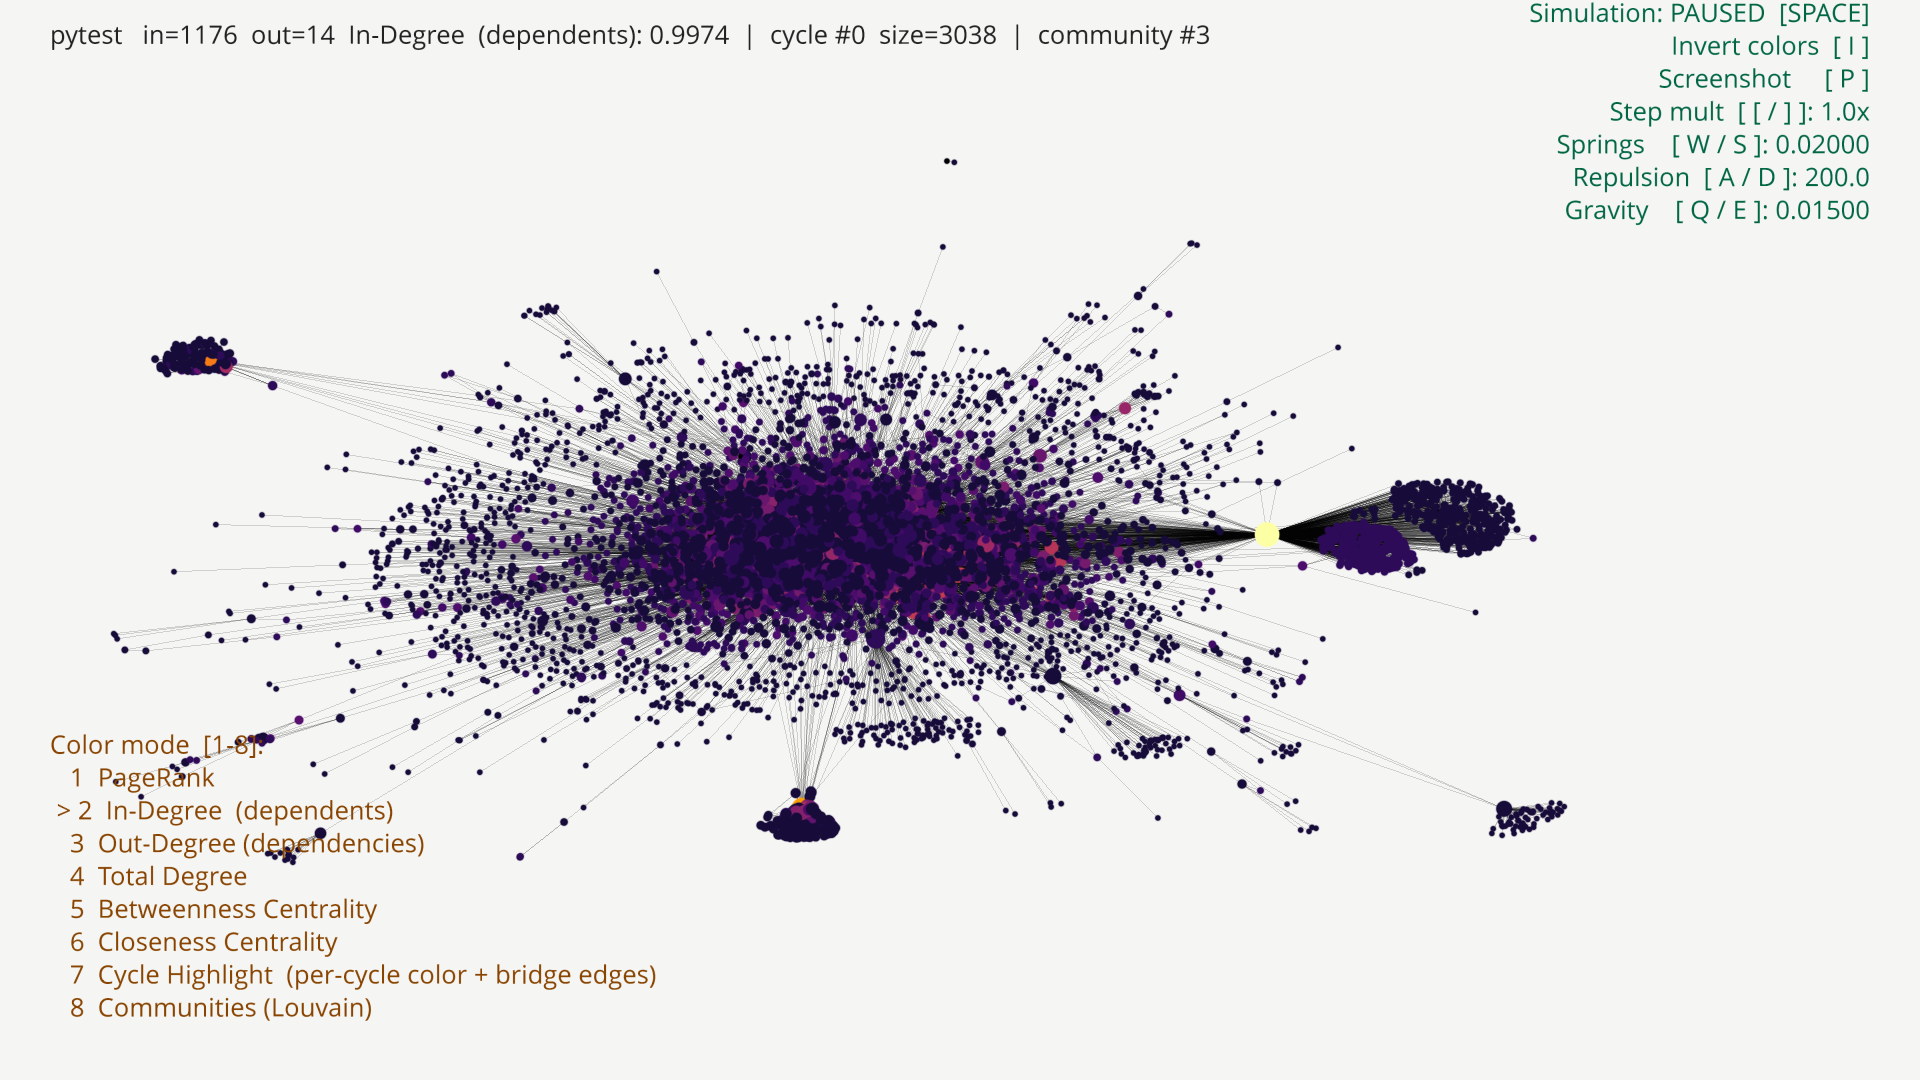
\includegraphics[width=1\linewidth]{Imagenes/IN_ALL}
		\caption{Representación del grado de entrada de los nodos de la red explotada en su totalidad.}
		\label{fig:inall}
	\end{figure}
	
	\begin{figure}[H]
		\centering
		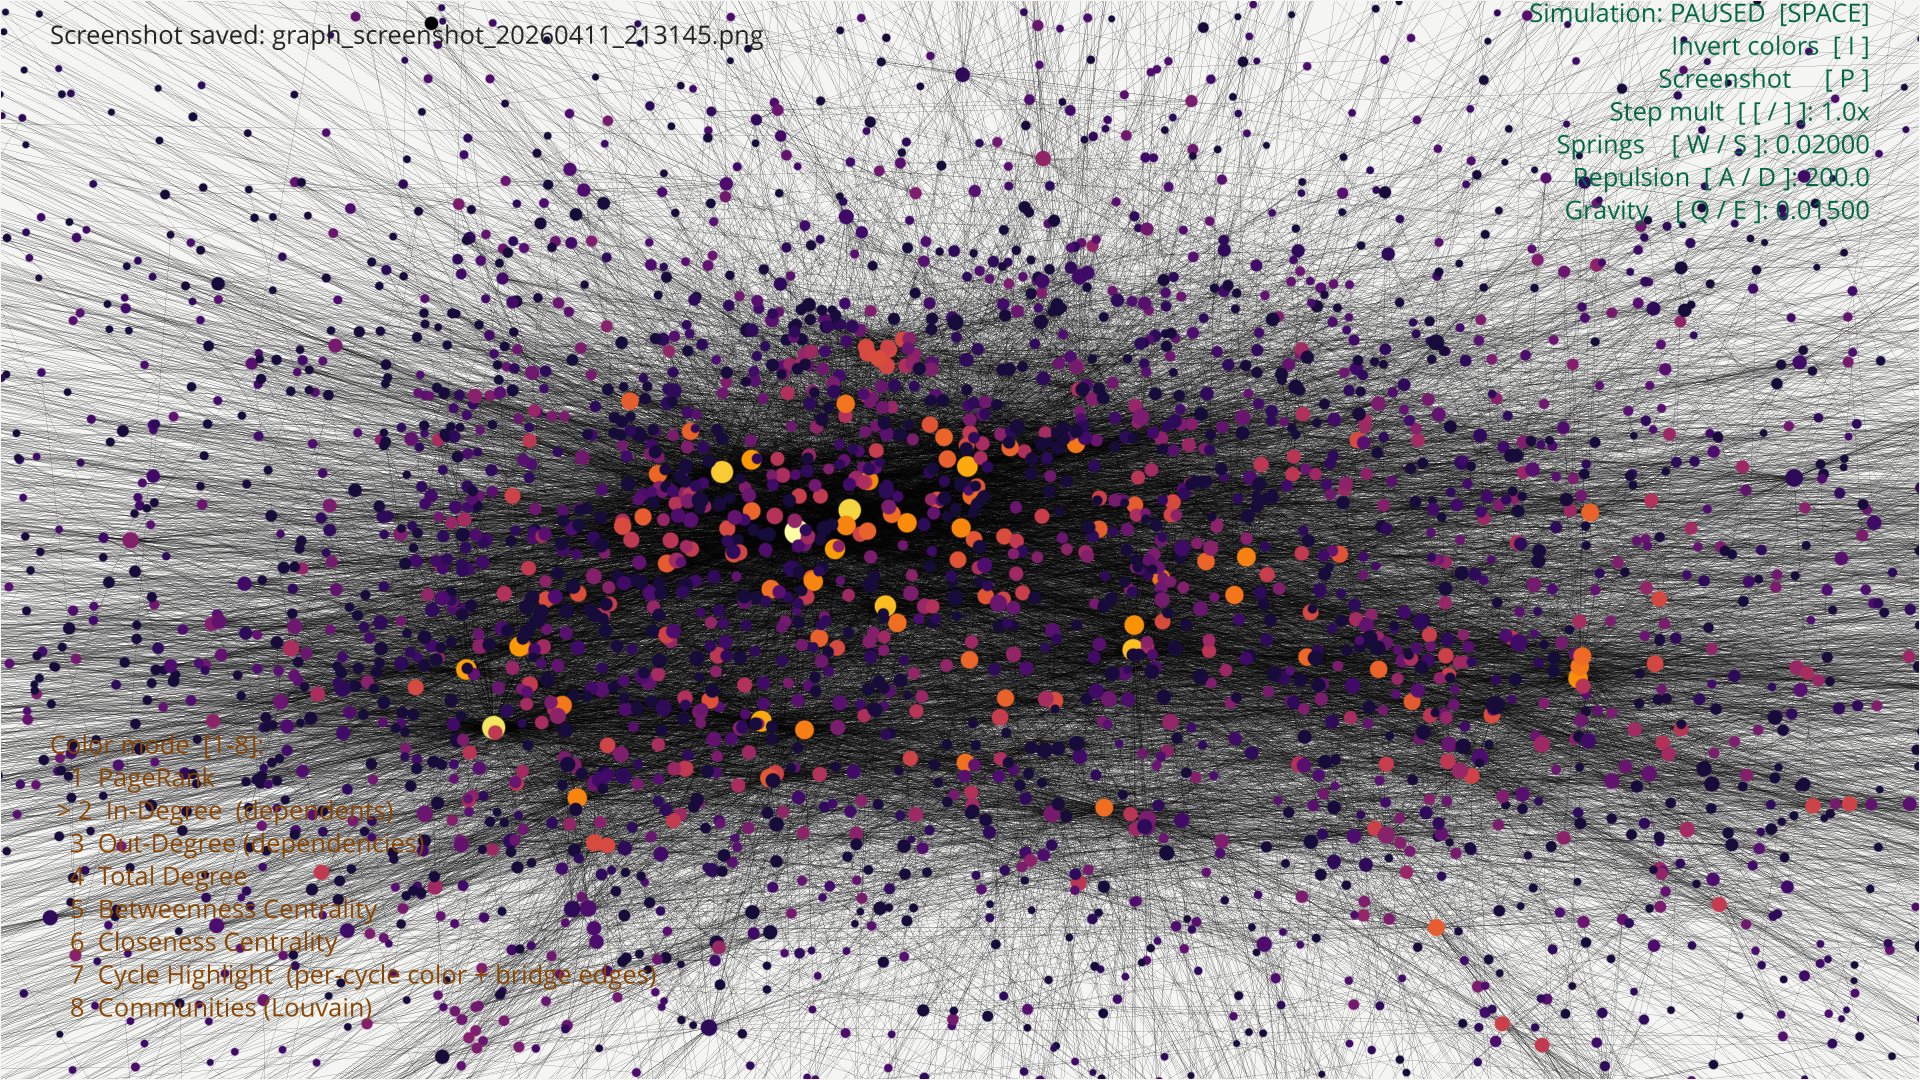
\includegraphics[width=1\linewidth]{Imagenes/IN_Center}
		\caption{Representación del grado de entrada de los nodos de la red explotada con zoom a la agrupación central.}
		\label{fig:incenter}
	\end{figure}
	
	\begin{figure}[H]
		\centering
		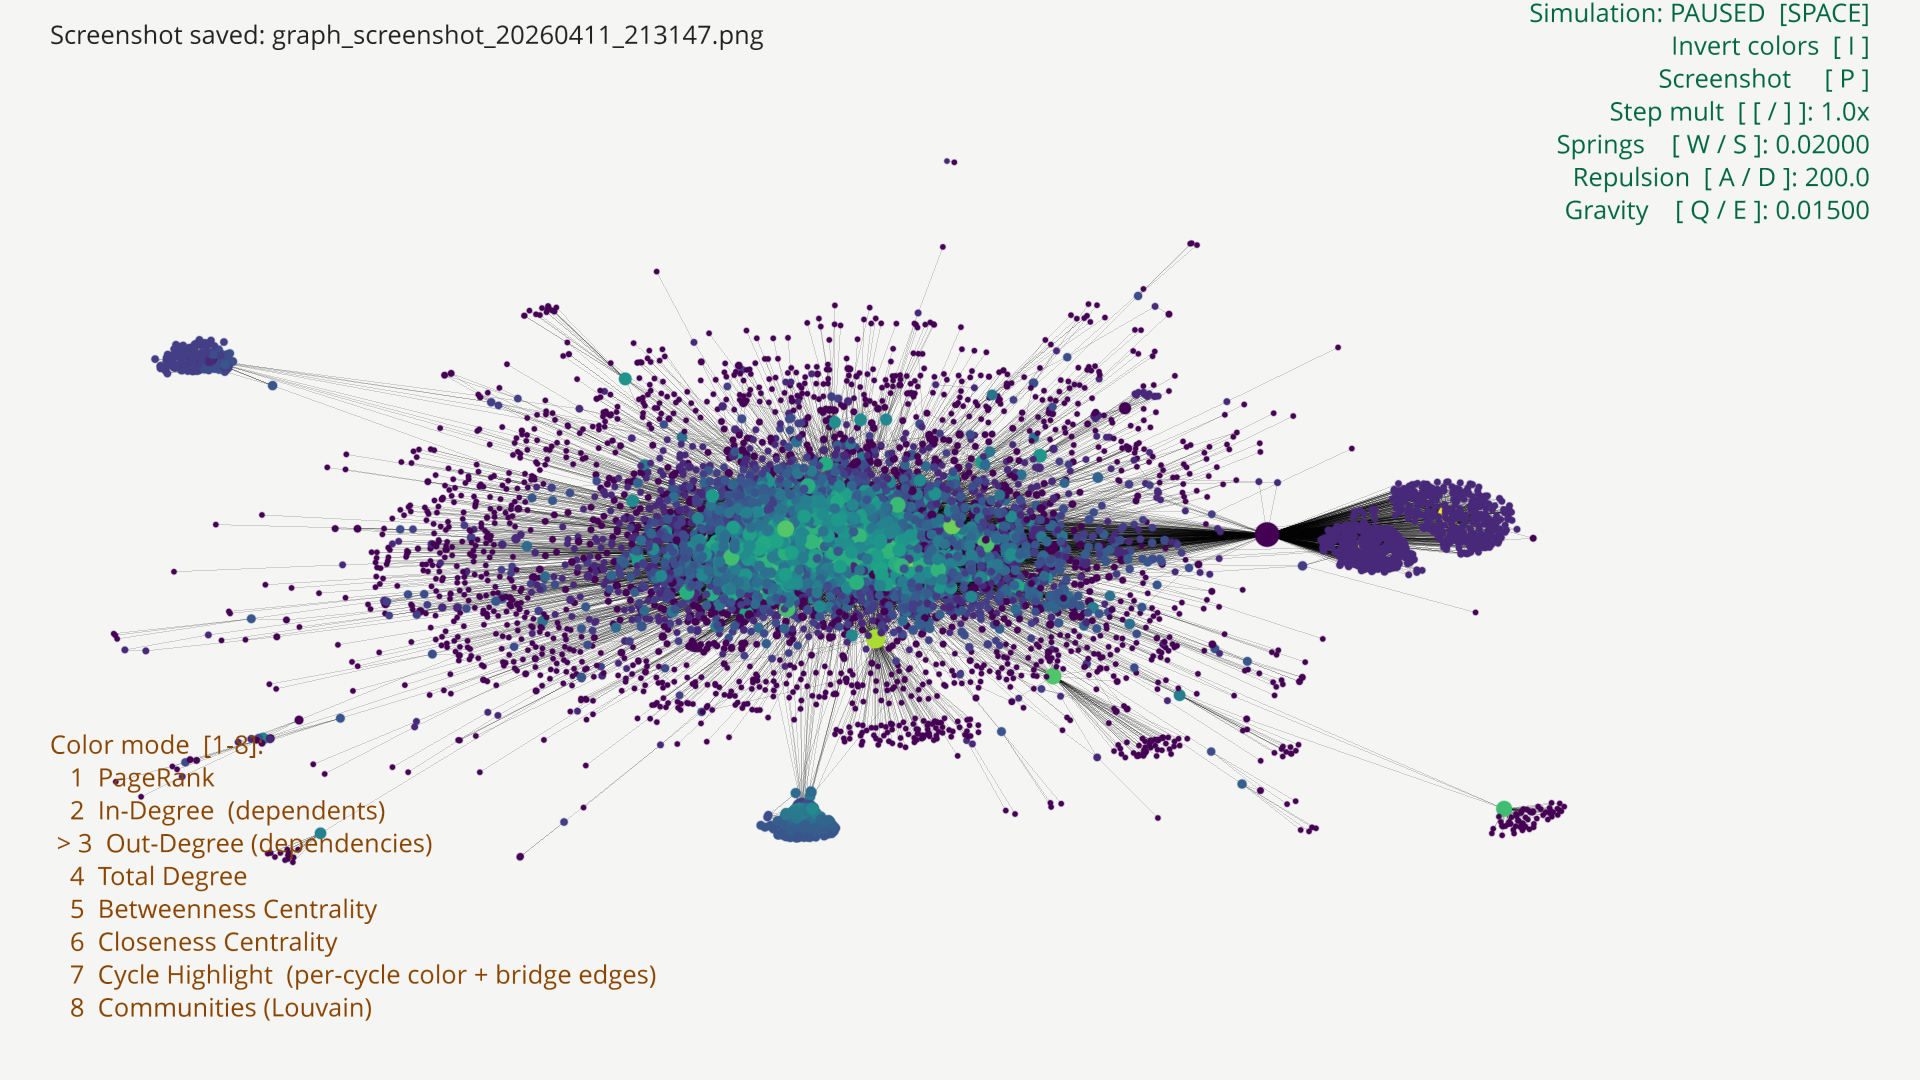
\includegraphics[width=1\linewidth]{Imagenes/OUT_ALL}
		\caption{Representación del grado de salida de los nodos de la red explotada en su totalidad.}
		\label{fig:outall}
	\end{figure}
	
	\begin{figure}[H]
		\centering
		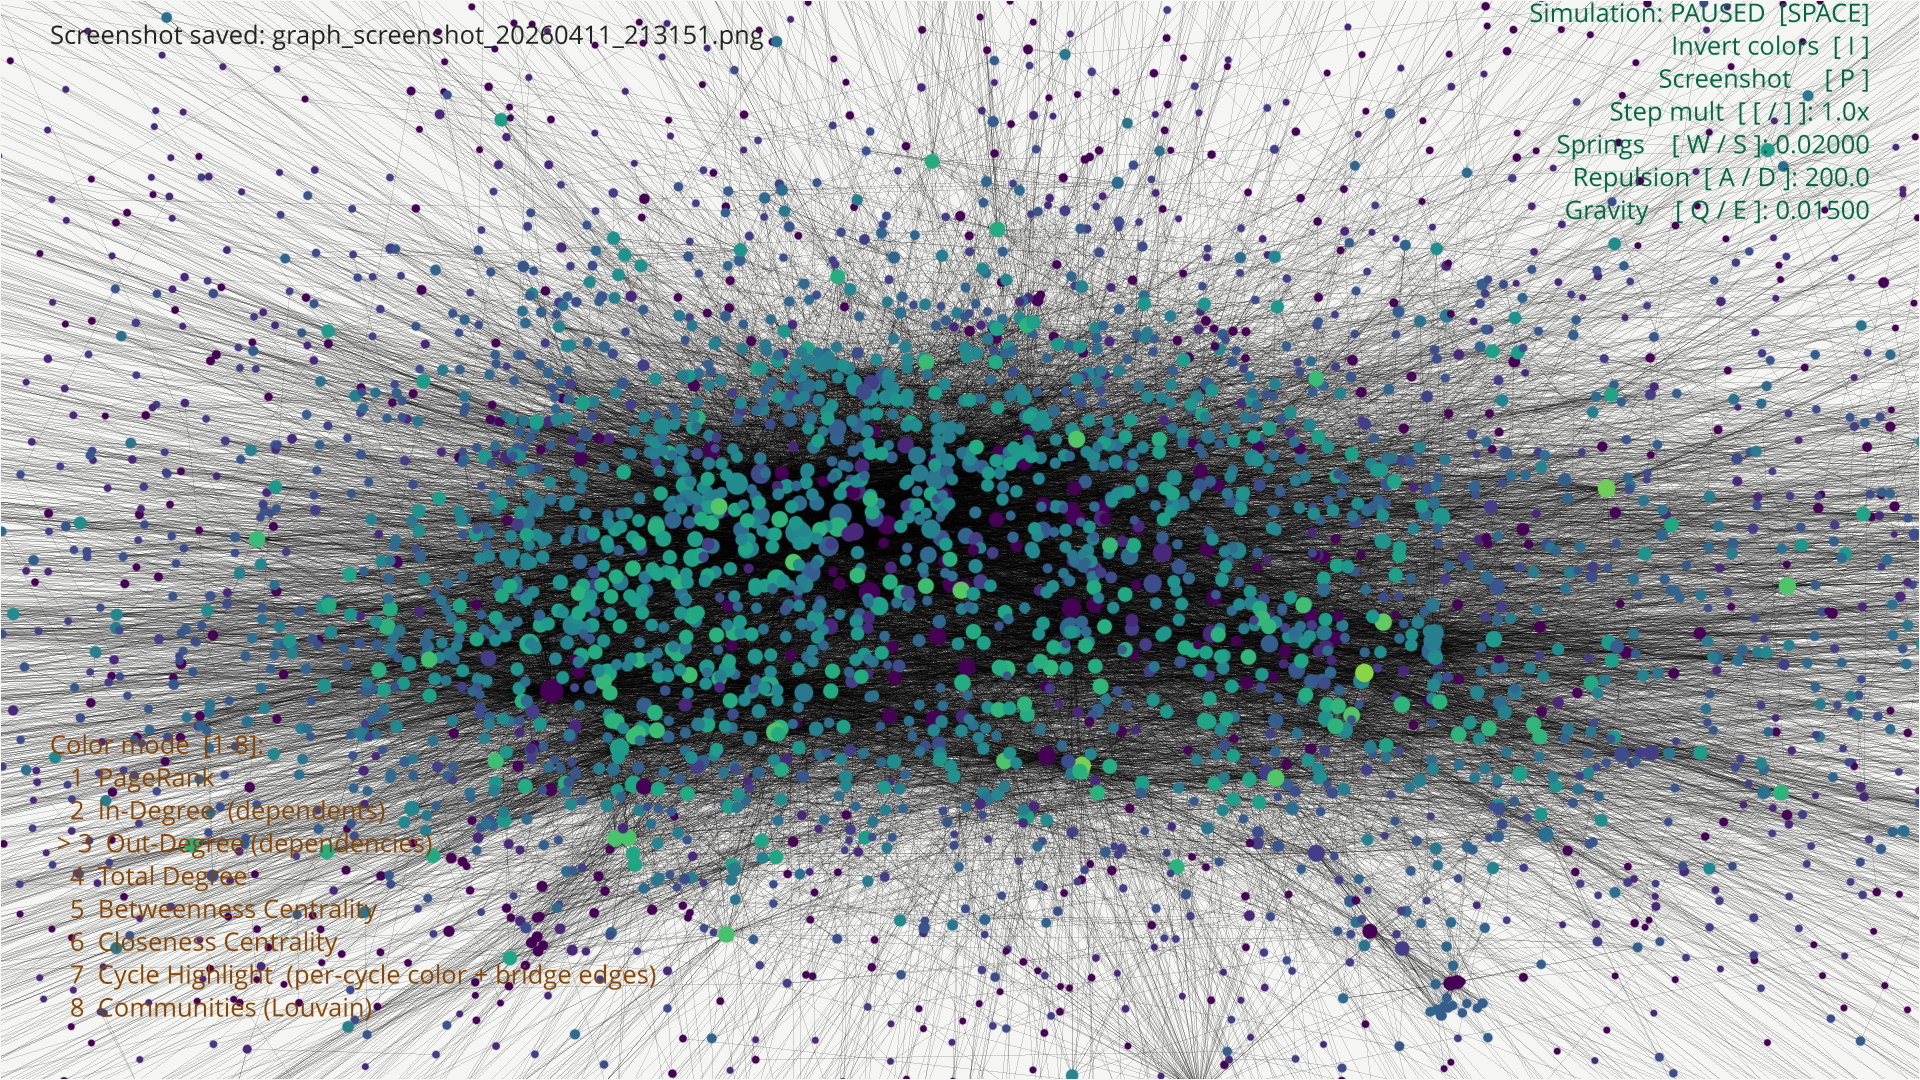
\includegraphics[width=1\linewidth]{Imagenes/OUT_center}
		\caption{Representación del grado de salida de los nodos de la red explotada con zoom a la agrupación central.}
		\label{fig:outcenter}
	\end{figure}
	
	De entre todos los nodos, un total de \(6763 (99.97\%)\) pertenecen a la componente gigante. Los paquetes \texttt{ansible} y \texttt{ansible-core\textasciitilde{}} pertenecen a una isla desconectada del resto del grafo. Resulta extraño que \texttt{ansible}, un paquete de automatización ampliamente utilizado en la industria para configurar servidores y servicios por lotes, no tenga dependencias de otros paquetes. La explicación se encuentra en la forma de construir la red. La dependencia de \texttt{ansible} es \texttt{ansible-core}, que a su vez depende de otros paquetes. No obstante, la expresión regular del parser no filtra adecuadamente el \textasciitilde{} y no encuentra el paquete \texttt{ansible-core\textasciitilde{}} porque no existe. Las figuras \ref{fig:conectedcomponent} y \ref{fig:conectedin} representan la componente gigante.
	
	\begin{figure}[H]
		\centering
		\includegraphics[width=1\linewidth]{Imagenes/ConectedComponent}
		\caption{Representación de la componente fuertemente conexa en rojo de la red explotada.}
		\label{fig:conectedcomponent}
	\end{figure}
	
	\begin{figure}[H]
		\centering
		\includegraphics[width=1\linewidth]{Imagenes/Conected_in}
		\caption{Representación de la componente fuertemente conexa en rojo con zoom en la agrupación central.}
		\label{fig:conectedin}
	\end{figure}
	
	La detección de islas se realiza analizando las componentes débilmente conexas, que no tienen en cuenta la dirección. Otro análisis interesante es el de las componentes fuertemente conexas. Se dice que la conexión entre dos nodos es fuerte si se puede ir y volver entre ellos. Este concepto está relacionado con la existencia de bucles. Si hay paquetes que se necesitan entre sí no se tiene un punto claro de inicio, por lo que la instalación no es limpia. Además, una actualización en uno de los paquetes podría provocar un cambio en el otro, y este cambio a su vez otro cambio en el paquete original. Este ciclo podría llegar a repetirse infinitamente. \\
	
	La cantidad de componentes fuertemente conexas debería ser igual al número de nodos (no hay paquetes que dependan mutuamente, por lo que no pueden formar una componente). En la red analizada hay 3727, lo que sugiere la existencia de ciclos. Solamente 2 componentes tienen más de un nodo. Es decir, hay 3725 paquetes sin dependencias cíclicas y los 3040 restantes se reparten entre 2 bucles. La longitud media de los bucles es de 1520 paquetes. Afinando el análisis, uno de los bucles contiene 2 nodos y el otro por 3038. El primero está compuesto por \texttt{ryd} y \texttt{ruamel.yaml}, dos paquetes de DevOps empleados para realizar lecturas y escrituras sobre archivos YAML. La composición del segundo es mucho más amplia como para analizar paquete a paquete. En la figura \ref{fig:pypi_ciclos_categorias} se han clasificado las librerías del bucle según la categoría a la que pertenecen utilizando un modelo de lenguaje. Cabe decir que dentro de la propia componente fuertemente conexa podría haber bucles internos, aunque este análisis no se ha realizado. Observando alguno de los paquetes en la componente fuertemente conexa, algunos de ellos resultan conocidos (por ejemplo, \texttt{fastapi}, \texttt{django} o \texttt{requests}) e incluso por experiencia al instalarlos no han arrastrado al resto de elementos en el bucle. La razón de este comportamiento es de nuevo atribuible a la construcción de la red, que no discrimina entre dependencias de producción o desarrollo. En producción, las instalaciones siguen una jerarquía de dependencias donde solamente se descargan los paquetes necesarios para el funcionamiento. En desarrollo, los autores de los paquetes base suelen declarar dependencias hacia paquetes de más alto nivel para comprobar que su código se integra correctamente con ellos. 
	
	\begin{figure}[H]
		\centering
		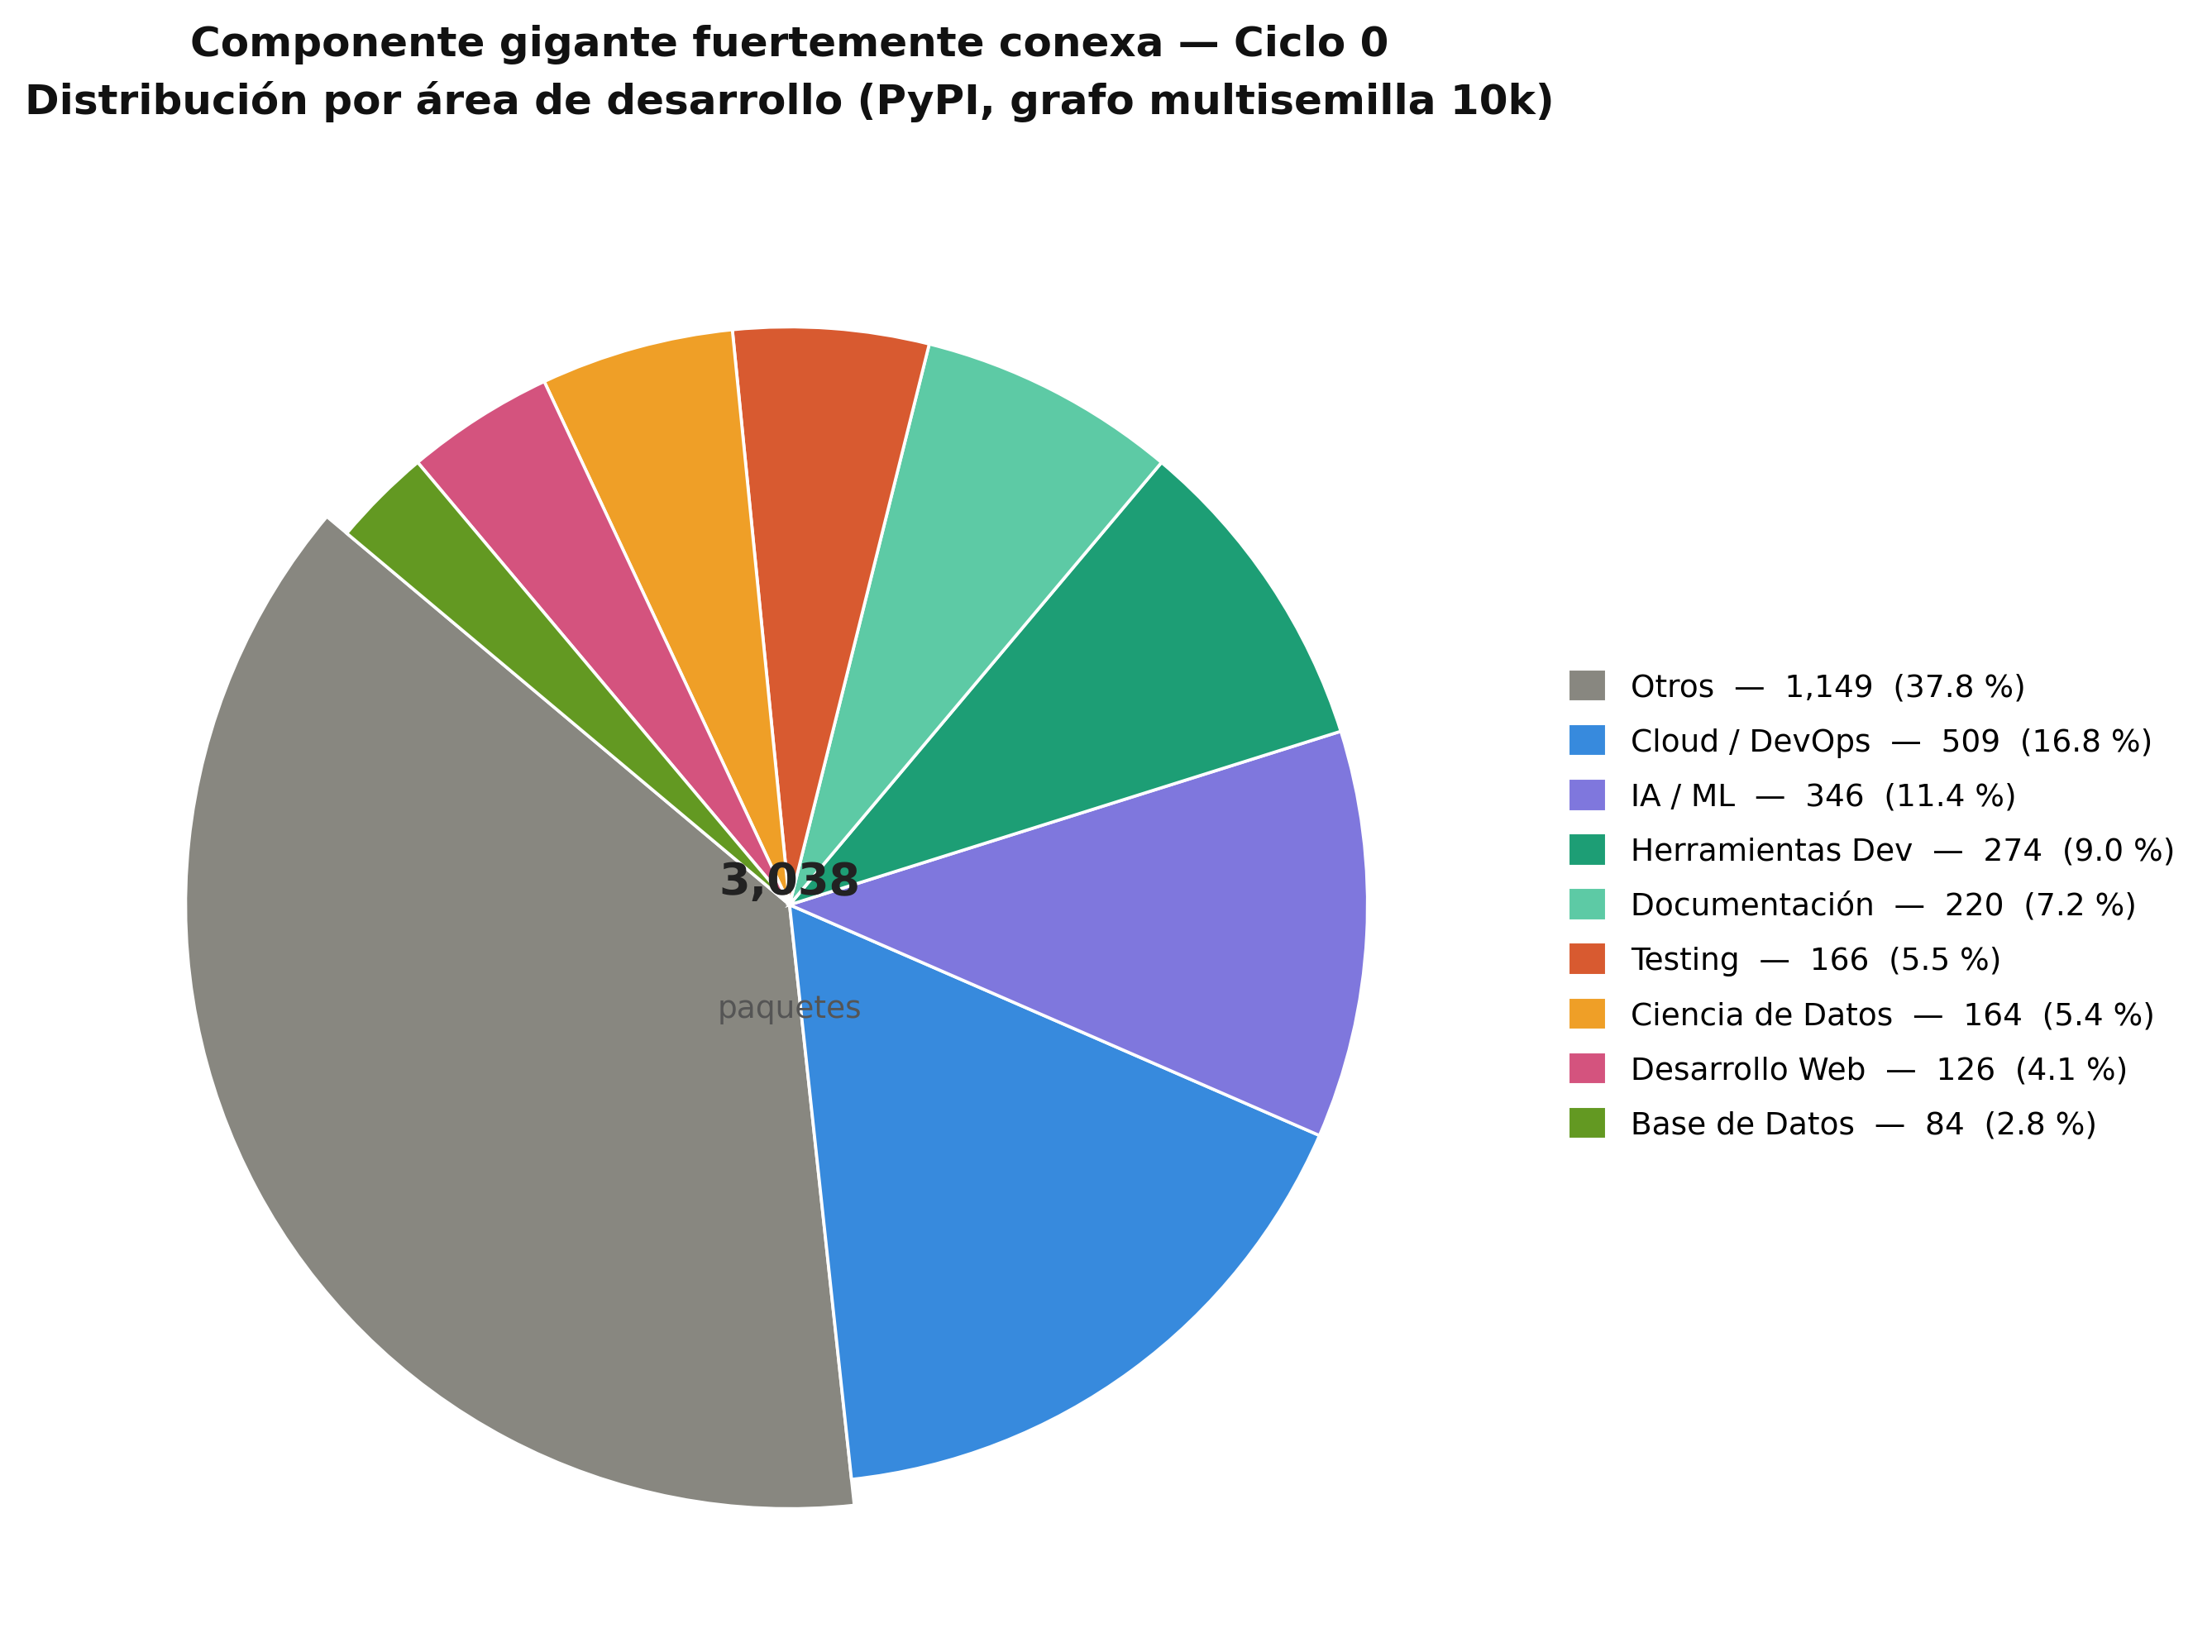
\includegraphics[width=0.8\linewidth]{Imagenes/pypi_ciclos_categorias.png}
		\caption{Categorización de los paquetes de PyPI en la componente fuertemente conexa.}
		\label{fig:pypi_ciclos_categorias}
	\end{figure}
	
	En la componente gigante extraída anteriormente se analizan algunas métricas adicionales. El diámetro es 25, lo que implica que en el peor de los casos esa será la profundidad de las dependencias de un paquete\footnote{No se debe asociar el diámetro al número de dependencias, sino a la profundidad de las mismas. Por ejemplo, un paquete podría depender de varios paquetes que no dependen de nadie más, en cuyo caso la profundidad sería 1 pero el número de dependencias sería mayor que 1.}. El radio se distingue según sea de entrada o de salida. El valor del primero es 6 y se relaciona con la accesibilidad de los paquetes básicos. Cualquier paquete dependiente del paquete menos excéntrico, lo alcanzará en un máximo de 6 pasos. El valor del segundo es 13 y se relaciona con la facilidad de instalar paquetes. En el mejor de los casos (paquete mejor posicionado), se requiere una instalación de profundidad 13.
	
	\subsection{Distribución de grado}
	Este apartado se ha realizado conforme al artículo \cite{Clauset_2009}. \\
	
	\subsubsection{Estimación de parámetros}
	El objetivo es verificar si la distribución de grado sigue una ley de potencias. Dado un valor $k_{mín}$ a partir del cual se empieza a cumplir la ley de potencias, se estima el valor de $\alpha$ por máxima verosimilitud resolviendo la ecuación:
	
	\begin{equation}
	\frac{\zeta'(\hat{\alpha}, x_{\min})}{\zeta(\hat{\alpha}, x_{\min})} = -\frac{1}{n} \sum_{i=1}^{n} \ln x_i
	\end{equation}
	
	donde $\zeta(\alpha, x_{mín})$ es la función zeta generalizada de Hurtwitz. En vez de resolver la ecuación anterior de forma numérica se puede obtener una aproximación a partir de la siguiente expresión:
	
	\begin{equation}
	\hat{\alpha} \approx 1 + n \left[\sum_{i=1}^n \ln \frac{x_i}{x_{mín} - 0.5}\right]
	\end{equation}
	
	donde $n$ es el número de paquetes en la cola y $x_i$ es el grado de la $i$-ésima observación. La desviación típica de $\hat{\alpha}$ en tiempo discreto se calcula con la fórmula:
	
	\begin{equation}
	\sigma = \frac{1}{\sqrt{n \left[ \frac{\zeta''(\hat{\alpha}, x_{min})}{\zeta(\hat{\alpha}, x_{min})} - \left( \frac{\zeta'(\hat{\alpha}, x_{min})}{\zeta(\hat{\alpha}, x_{min})} \right)^2 \right]}}
	\end{equation}
	
	No obstante, si el número de nodos en la cola es alto se puede aproximar por:
	
	\begin{equation}
	\hat{\sigma} \approx \frac{\hat{\alpha} - 1}{\sqrt{n}}
	\end{equation}
	
	La elección del valor de $x_{mín}$ se hace por \textit{grid search}. Es decir, se obtiene el estimador de máxima verosimilitud de $\alpha$ para cada valor posible de $x_{mín}$ y se selecciona el que minimice el estadístico de Kolmogorov-Smirnov:
	
	\begin{equation}
	KS = \max_{x \ge x_{mín}} |S(x) - P(x)|
	\end{equation} 
	
	donde $S(x)$ es la función de distribución empírica de la cola de los datos disponibles y $P(x)$ es la función de distribución teórica de la ley de potencias. Si el valor de $x_{mín}$ es alto se tendrán pocos valores en la cola y el ajuste será deficiente debido al ruido estadístico. Si es bajo, se estará modelando el parte del cuerpo y la cola con una distribución que describe solo la cola. Entre medias se encuentra el valor óptimo que se pretende estimar, $\hat{x}_{mín}$. \\
	
	La incertidumbre asociada a $\hat{x}_{mín}$ se cuantifica empleando \textit{bootstrapping} no paramétrico. Se construyen conjuntos de datos sintéticos mediante muestreo con reemplazo sobre el conjunto original y se busca $\hat{x}_{mín}$ en cada caso con el método explicado anteriormente. La incertidumbre asociada a $\hat{x}_{mín}$ es la desviación típica sobre los conjuntos sintéticos. 
	
	\subsubsection{Tests de bondad de ajuste}	
	Los métodos anteriores no explican la plausibilidad de la ley de potencias calculada. El problema es complejo por dos razones. La primera es que incluso las propias realizaciones a partir de una ley de potencias dadas podrían no seguir dicha ley debido al proceso de muestreo. La segunda es que se pueden dar casos en los que la red proviene de otra distribución pero su realización particular sigue una ley de potencias. Se busca plantear un test de bondad de ajuste que permita discriminar entre fluctuaciones aleatorias asociadas al muestreo y distribuciones distintas. El procedimiento se basa en generar varios conjuntos de datos sintéticos y calcular la proporción de veces que el estadístico de Kolmogorov-Smirnov es menor en los datos empíricos que en los generados artificialmente. Este cociente es el p-valor. \\
	
	El contraste anterior es semiparamétrico, dado que con probabilidad $\frac{n_{cola}}{n}$, con $n_{cola}$ el número de observaciones en la cola dado el punto de corte $\hat{x}_{mín}$, se generan datos de acuerdo a la ley de potencias y el resto se seleccionan aleatoriamente del cuerpo de los datos originales. Para cada conjunto sintético se reajustan los valores de $\hat{x}_{mín}$ y $\hat{\alpha}$ con el fin de seguir el mismo procedimiento que se siguió con la red original\footnote{Si la red original proviniera de una ley de potencias, pero los datos en el cuerpo se alinearan con los de la cola, el estadístico KS sería más bajo de lo que debería. Por lo tanto, el p-valor estaría inflado debido a que el sobreajuste provoca un error menor que el que tendrían los datos sintéticos al medirse sobre la ley que los generó. Para que la comparación sea justa, los parámetros de la ley de potencias deben reajustarse.}. Para muestrear de una ley de potencias discreta, habría que aplicar el método de la transformada inversa sobre:
	
	\begin{equation}
	P(x) = \sum_{x'=x}^{\infty}p(x') = 1 - r
	\end{equation}
	
	donde $r \sim U(0,1)$. La fórmula anterior no es invertible, por lo que debe resolverse numéricamente. Una alternativa es utilizar una aproximación:
	
	\begin{equation}
	x = \left\lfloor \left(x_{\min} - \frac{1}{2}\right)(1 - r)^{-1/(\alpha - 1)} + \frac{1}{2} \right\rfloor
	\end{equation}
	
	\subsubsection{Comparación con distribuciones alternativas}
	Incluso si la ley de potencias ajusta adecuadamente la distribución de grado, podría haber distribuciones que lo hicieran mejor. La forma de proceder es obtener la distribución alternativa que mejor se ajusta a los datos y comparar el cociente de log-verosimilitudes, $\mathcal{R}$. Si $\mathcal{R}$ es positivo, la ley de potencias se ajustará mejor a los datos, mientras que si es negativo será la distribución alternativa. Si es cercano a 0 significa que ha habido un empate. El signo de $\mathcal{R}$ podría deberse meramente al ruido estadístico, por lo que se debe calcular su valor esperado. Otro aspecto a tener en cuenta consiste en determinar qué significa que $\mathcal{R}$ esté cerca o lejos de 0. La respuesta viene del test de Voung. \\
	
	A continuación, se expone el formalismo matemático:
	
	\begin{equation}
	\left.
	\begin{aligned}
	& L_1 = \prod_{i=1}^n p_1(x_i) \\
	& L_2 = \prod_{i=1}^n p_2(x_i) \\
	& R = \frac{L_1}{L_2} = \prod_{i=1}^n \frac{p_1(x_i)}{p_2(x_i)}
	\end{aligned}
	\right\} \implies \mathcal{R} = \sum_{i=1}^n \left[\ln p_1(x_i) - \ln p_2(x_i)\right] = \sum_{i=1}^{n}\left[\ell_i^{(1)} - \ell_i^{(2)}\right]
	\end{equation}
	
	Dado que las muestras $x_i$ son independientes, las diferencias $\ell_i^{(1)} - \ell_i^{(2)}$ también lo son. Aplicando el teorema central del límite $\mathcal{R}$ se distribuye como una normal con varianza $n \sigma^2$, donde $\sigma^2$ es la varianza de un término que se puede aproximar por la varianza muestral:
	
	\begin{align}
	& \sigma^2 = \frac{1}{n}\sum_{i=1}^n\left[\left(\ell_i^{(1)} - \ell_i^{(2)}\right) - \left(\hat{\ell}^(1) - \hat{\ell}^{(2)}\right)\right] \\
	& \hat{\ell}^{(1)} = \frac{1}{n} \sum_{i=1}^n \ell_i^{(1)} \\
	& \hat{\ell}^{(2)} = \frac{1}{n} \sum_{i=1}^n \ell_i^{(2)}
	\end{align}
	
	Si las distribuciones son iguales, la diferencia de log-verosimilitudes es 0, que se toma como hipótesis nula. Esta se rechazará si la probabilidad de obtener la diferencia de log-verosimilitudes observada es menor que un determinado valor:
	
	\begin{equation}
	p = \frac{1}{\sqrt{2\pi n \sigma^2}}\left[\int_{-\infty}^{-|R|}e^{-\frac{t^2}{2n\sigma^2}} dt + \int_{|R|}^{\infty}e^{-\frac{t^2}{2n\sigma^2}} dt\right]
	\end{equation}
	
	\subsubsection{Resultados}
	La tabla \ref{tab:res_dgrado} resume el ajuste de los parámetros de la ley de potencias y la simulación de Monte Carlo para evaluar la bondad del ajuste en la distribución de los grados de entrada y salida de la red. La hipótesis de distribución bajo una ley de potencias se verifica para el grado de entrada pero se rechaza para el de salida. Esto es coherente con la idea de que si alguien desarrolla un nuevo paquete, este dependa de los paquetes populares antes que de los desconocidos. Sin embargo, un paquete con muchas dependencias no va a depender de nuevos paquetes que se incorporen a la red (principalmente porque ya podía funcionar sin dichos paquetes). \\
	
	El valor de $\hat{x}_{mín}$ también puede ser indicador del cumplimiento de la ley de potencias. Para el grado de entrada se mantiene en el rango $[2, 4]$ mientras que para el de salida las fluctuaciones son mayores. Además, el estadistico KS es 6 más alto en la segunda distribución. Cabe decir que $\alpha < 2$ para la distribución de grado de entrada, lo que implica que todos los momentos divergen, incluidos la media y la varianza. Por lo tanto, no se puede hablar de grado medio.
	
	\begin{table}[H]
		\centering
		\begin{tabular}{lcc}
			\toprule
			\textbf{Métrica} & \textbf{Grado de Entrada} & \textbf{Grado de Salida} \\
			\midrule
			$x_{\min}$ óptimo & 3.0 & 11.0 \\
			$x_{\min}$ bootstrap & $3.6 \pm 1.4$ & $21.4 \pm 8.9$ \\
			$\alpha$ óptimo & $1.8999 \pm 0.0222$ & $2.5158 \pm 0.0479$ \\
			KS óptima & 0.0139 & 0.0608 \\
			$n_{\text{cola}}$ & 1646 (24.3\%) & 1001 (22.0\%) \\
			p-valor (Test KS) & 0.532 & 0.000 \\
			\midrule
			Test de Vuong & No rechazada ($p > 0.1$) & Rechazada ($p \le 0.1$) \\
			\bottomrule
		\end{tabular}
		\caption{Resumen del ajuste de ley de potencias para los grados de entrada y salida.}
		\label{tab:res_dgrado}
	\end{table}
	
	La figura \ref{fig:dgrado} muestra las distribuciones de masa de probabilidad empírica y teórica de los grados de entrada y salida de la red. Visualmente, el ajuste parece mejor para el grado de entrada. Hay que enfatizar que la distribución teórica se calcula solo para los datos de la cola, los cuales representa una fracción de la probabilidad total. Si se dibuja la ley de potencias calculada directamente saldrá por encima de la nube de puntos. Esto es porque la línea negra acumulará toda la probabilidad y tendrá más para repartir a cada punto. Para corregir el efecto, se debe multiplicar la probabilidad de grado teórica por la probabilidad de pertenecer a la cola ($\frac{n_{cola}}{n}$). También se ve cómo a partir de un determinado grado la probabilidad de la distribución empírica se estanca, mientras que la de la teórica sigue decreciendo. La razón es el número limitado de observaciones disponibles. Los paquetes con un elevado número de dependencias aparecen una vez en la red, sin importar cuál sea ese número. Por lo tanto, la probabilidad que acumulan es la misma. Si hubiera más muestras se seguiría la ley de potencias más allá de lo que se ve en la imagen. Finalmente, a la derecha se representa el valor del estadístico KS según el valor de corte $\hat{x}_{mín}$. 
	
	\begin{figure}[H]
		\centering
		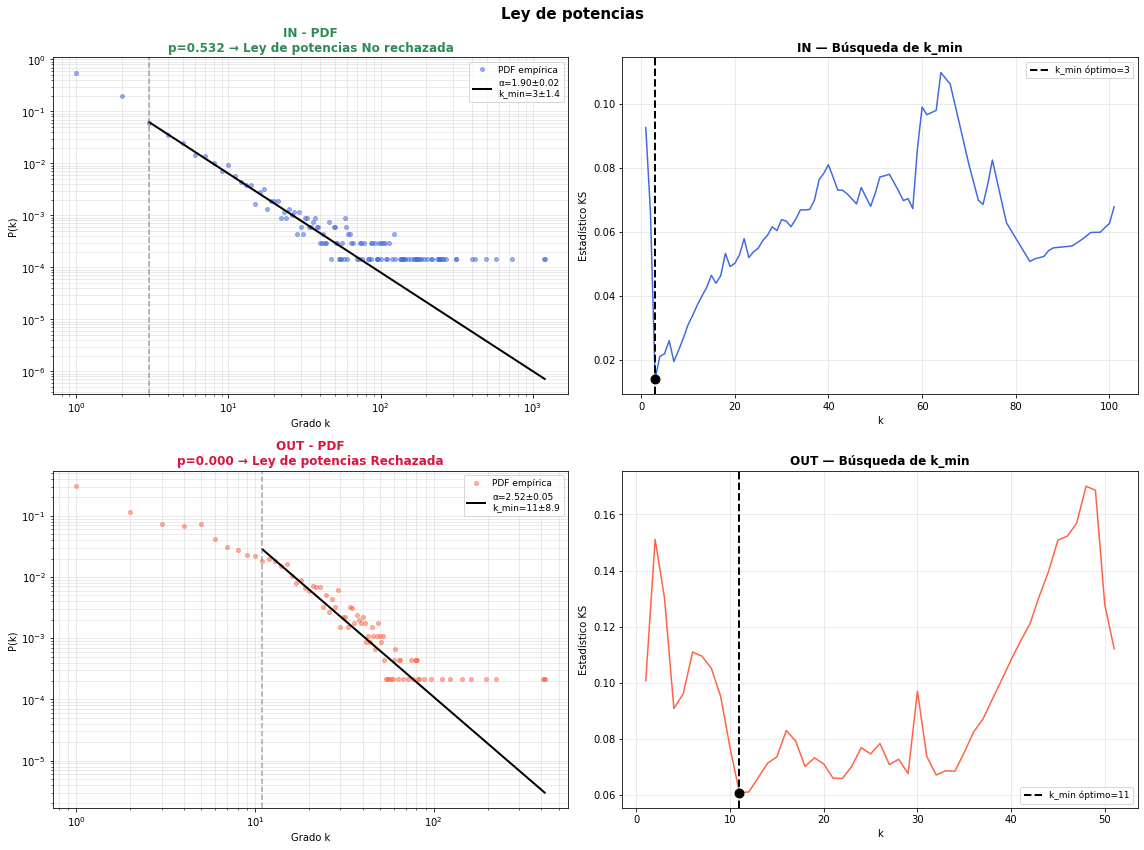
\includegraphics[width=1\linewidth]{Imagenes/ley_potencias_kmin}
		\caption{Distribuciones de masa de probabilidad empíricas y teóricas y proceso de búsqueda de $x_{mín}$ óptimo para los grados de entrada y salida.}
		\label{fig:dgrado}
	\end{figure}
	
	La distribución según ley de potencias se compara con las presentadas en la tabla \ref{tab:dist_alternativas}. En la tabla \ref{tab:likelihood_ratio_test} se resumen los tests de razón de verosimilitud entre la ley de potencias y las distribuciones alternativas. Aunque para la distribución de grado de salida no tiene demasiado sentido porque se rechazó la hipótesis de que siguen una ley de potencias, la comparación sugiere que una Yule podría funcionar mejor. Para la distribución de entrada, la ley de potencias resulta favorable frente a la exponencial y la Poisson, mientras que es indistinguible de la Yule.
	
	\begin{table}[H]
		\centering
		\renewcommand{\arraystretch}{2.2} % Aumenta el espacio vertical para que no se aplasten las fracciones
		\begin{tabular}{ll}
			\toprule
			\textbf{Distribución} & \textbf{Ecuaciones (PMF y log-verosimilitud)} \\
			\midrule
			% EXPONENCIAL
			\multirow{2}{*}{\textbf{Exponencial}} 
			& $p(x) = (1 - e^{-\lambda}) e^{\lambda x_{\min}} e^{-\lambda x}$ \\
			& $\ell(x) = \ln(1 - e^{-\lambda}) + \lambda x_{\min} - \lambda x$ \\
			\midrule
			% YULE
			\multirow{2}{*}{\textbf{Yule}} 
			& $p(x) = (\alpha - 1) \frac{\Gamma(x_{\min} + \alpha - 1)}{\Gamma(x_{\min})} \frac{\Gamma(x)}{\Gamma(x + \alpha)}$ \\
			& $\ell(x) = \ln(\alpha - 1) + \ln\Gamma(x_{\min} + \alpha - 1) - \ln\Gamma(x_{\min}) + \ln\Gamma(x) - \ln\Gamma(x + \alpha)$ \\
			\midrule
			% POISSON
			\multirow{2}{*}{\textbf{Poisson}} 
			& $p(x) = \left[ e^{\mu} - \sum_{k=0}^{x_{\min}-1} \frac{\mu^k}{k!} \right]^{-1} \frac{\mu^x}{x!}$ \\
			& $\ell(x) = x \ln(\mu) - \ln\Gamma(x + 1) - \ln\left( e^{\mu} - \sum_{k=0}^{x_{\min}-1} \frac{\mu^k}{k!} \right)$ \\
			\bottomrule
		\end{tabular}
		\caption{Funciones de masa de probabilidad y log-verosimilitud para distribuciones discretas alternativas a la ley de potencias: exponencial, Yule y Poisson.}
		\label{tab:dist_alternativas}
	\end{table}
	
	\begin{table}[H]
		\centering
		\begin{tabular}{lrcl}
			\toprule
			\textbf{Distribución Alternativa} & \textbf{LR ($\mathcal{R}$)} & \textbf{p-valor} & \textbf{Interpretación} \\
			\midrule
			\multicolumn{4}{c}{\textbf{Grado de Entrada} \quad ($k_{\min}=3$, $\alpha=1.900$, $p_{\text{KS}}=0.532$)} \\
			\midrule
			Exponencial & $8.432$ & $<0.001$ & Ley de potencias favorable \\
			Poisson     & $5.401$ & $<0.001$ & Ley de potencias favorable \\
			Yule        & $-1.598$ & $0.110$ & No distinguibles \\
			\midrule
			\multicolumn{4}{c}{\textbf{Grado de Salida} \quad ($k_{\min}=11$, $\alpha=2.516$, $p_{\text{KS}}<0.001$)} \\
			\midrule
			Exponencial & $1.307$ & $0.191$ & No distinguibles \\
			Poisson     & $3.824$ & $<0.001$ & Ley de potencias favorable \\
			Yule        & $-8.943$ & $<0.001$ & Alternativa favorable \\
			\bottomrule
		\end{tabular}
		\caption{Tests de razón de verosimilitud entre la ley de potencias empírica y las distribuciones alternativas para la región de la cola.}
		\label{tab:likelihood_ratio_test}
	\end{table}

	\section{Análisis de centralidad}
	Una vez realizado el análisis preliminar de la red se estudian las propiedades de centralidad de la misma para ver qué paquetes son los más importantes dentro de la red de dependencias de Python. Para realizar este estudio se estudian las tres magnitudes estudiadas en clase: PageRank, Centralidad de Intermediación y Centralidad de Cercania mediante el script \texttt{centrality.py}. Estos nodos son 
	
	


	\subsection{PageRank}
	Como se trabaja con un grafo dirigido, esta medida de centralidad es de aplicación directa al análisis de trabajo. En este contexto, el PageRank representa la probabilidad de alcanzar un paquete dado mediante un paseo aleatorio de Markov a través del grafo, utilizando un factor de salto de $\theta=0.85$. Por tanto, puede entenderse que aquellos paquetes que acaben con un valor más alto de esta métrica serán los más relevantes de la red de dependencias de Python.
	\newline
	
	Visualmente, tal y como se puede ver en las figuras \ref{fig:pagerankfull} y \ref{fig:pagerankin} se ven varios nodos que destacan en importancia. Además, la ejecución del script \texttt{centrality.py} confirma que hay dos nodos, \texttt{typing-extensions} y \texttt{pytest}, que presentan una ponderación logarítmica muy superior al resto. Estos son seguidos por paquetes donde ya la distancia en PageRank entre ellos ya no es tan grande.
	
	
	
	\begin{figure}[H]
		\centering
		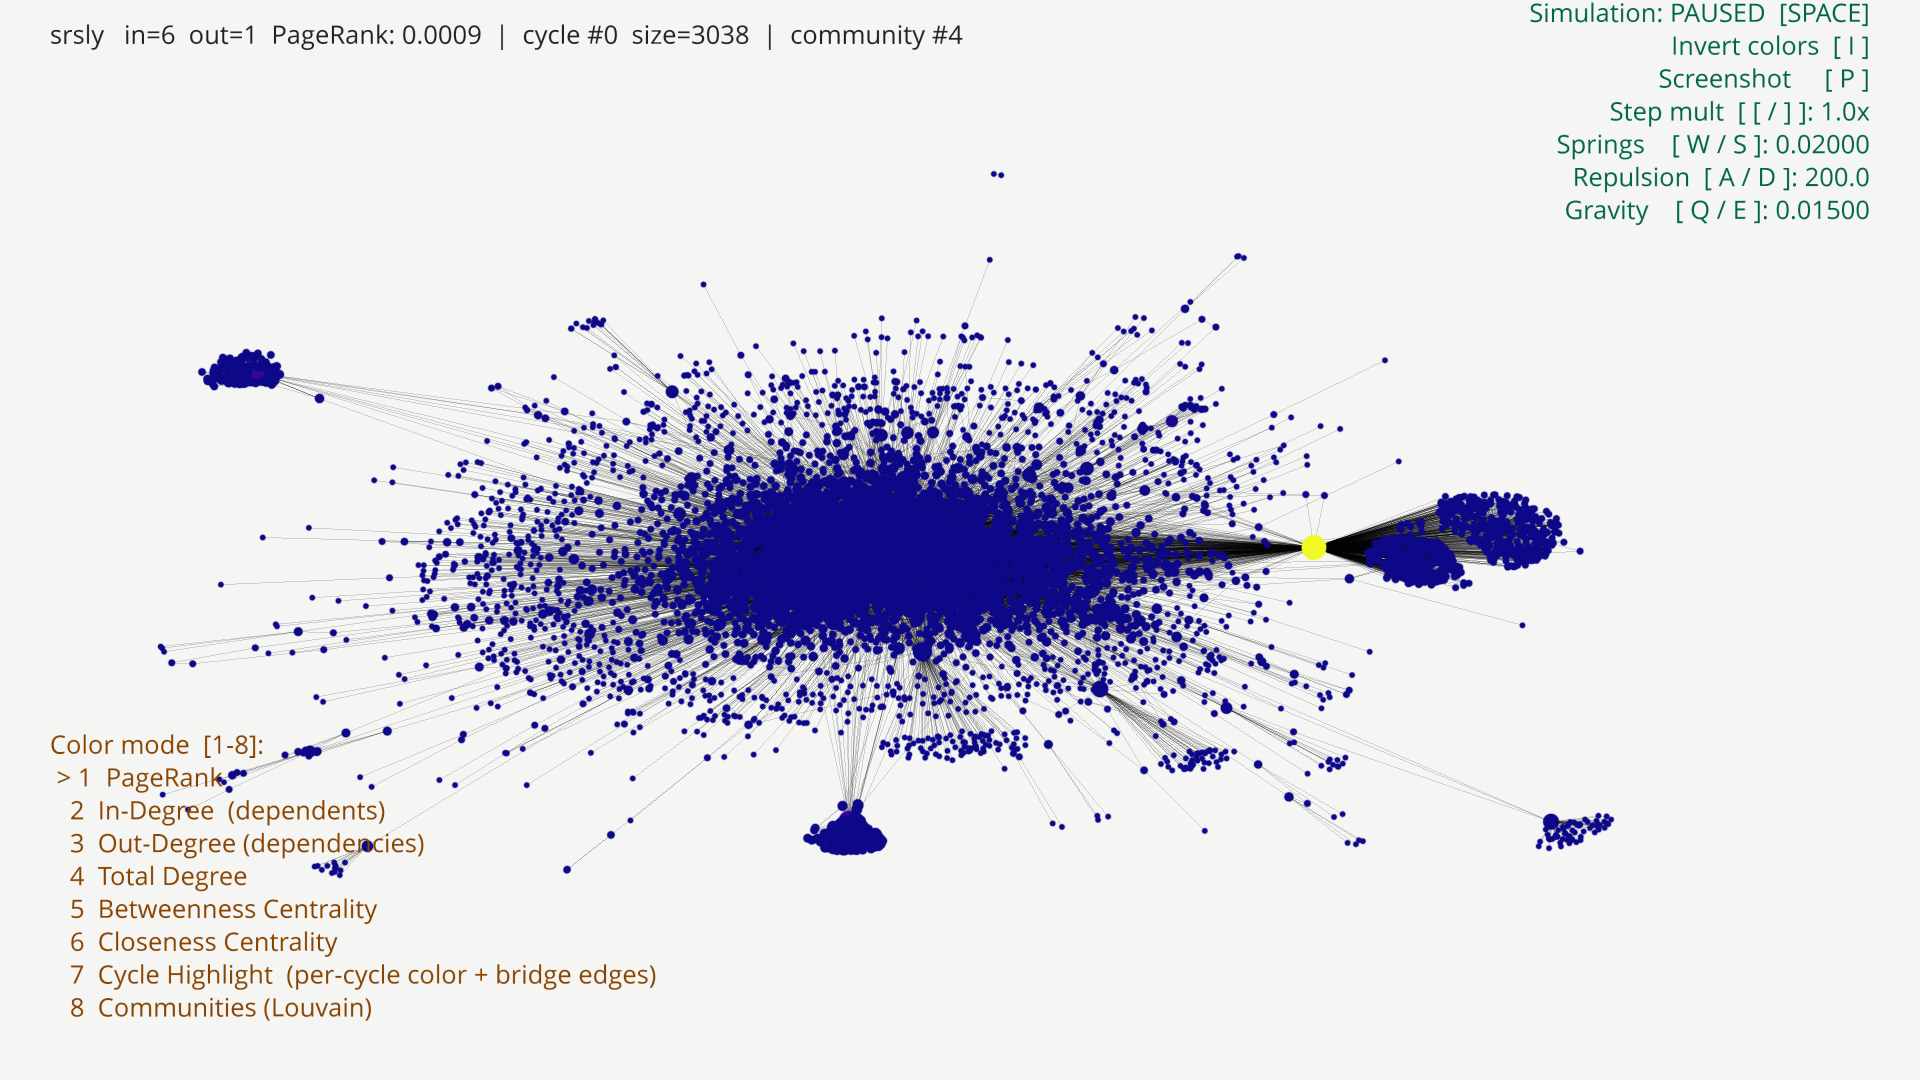
\includegraphics[width=1\linewidth]{Imagenes/PageRank_full}
		\caption{Representación del PageRank en la red completa de dependencias de Python donde en amarillo están los paquetes con mayor valor de esta métrica y en azul aquellos con menor valor.}
		\label{fig:pagerankfull}
	\end{figure}
	\begin{figure}[H]
		\centering
		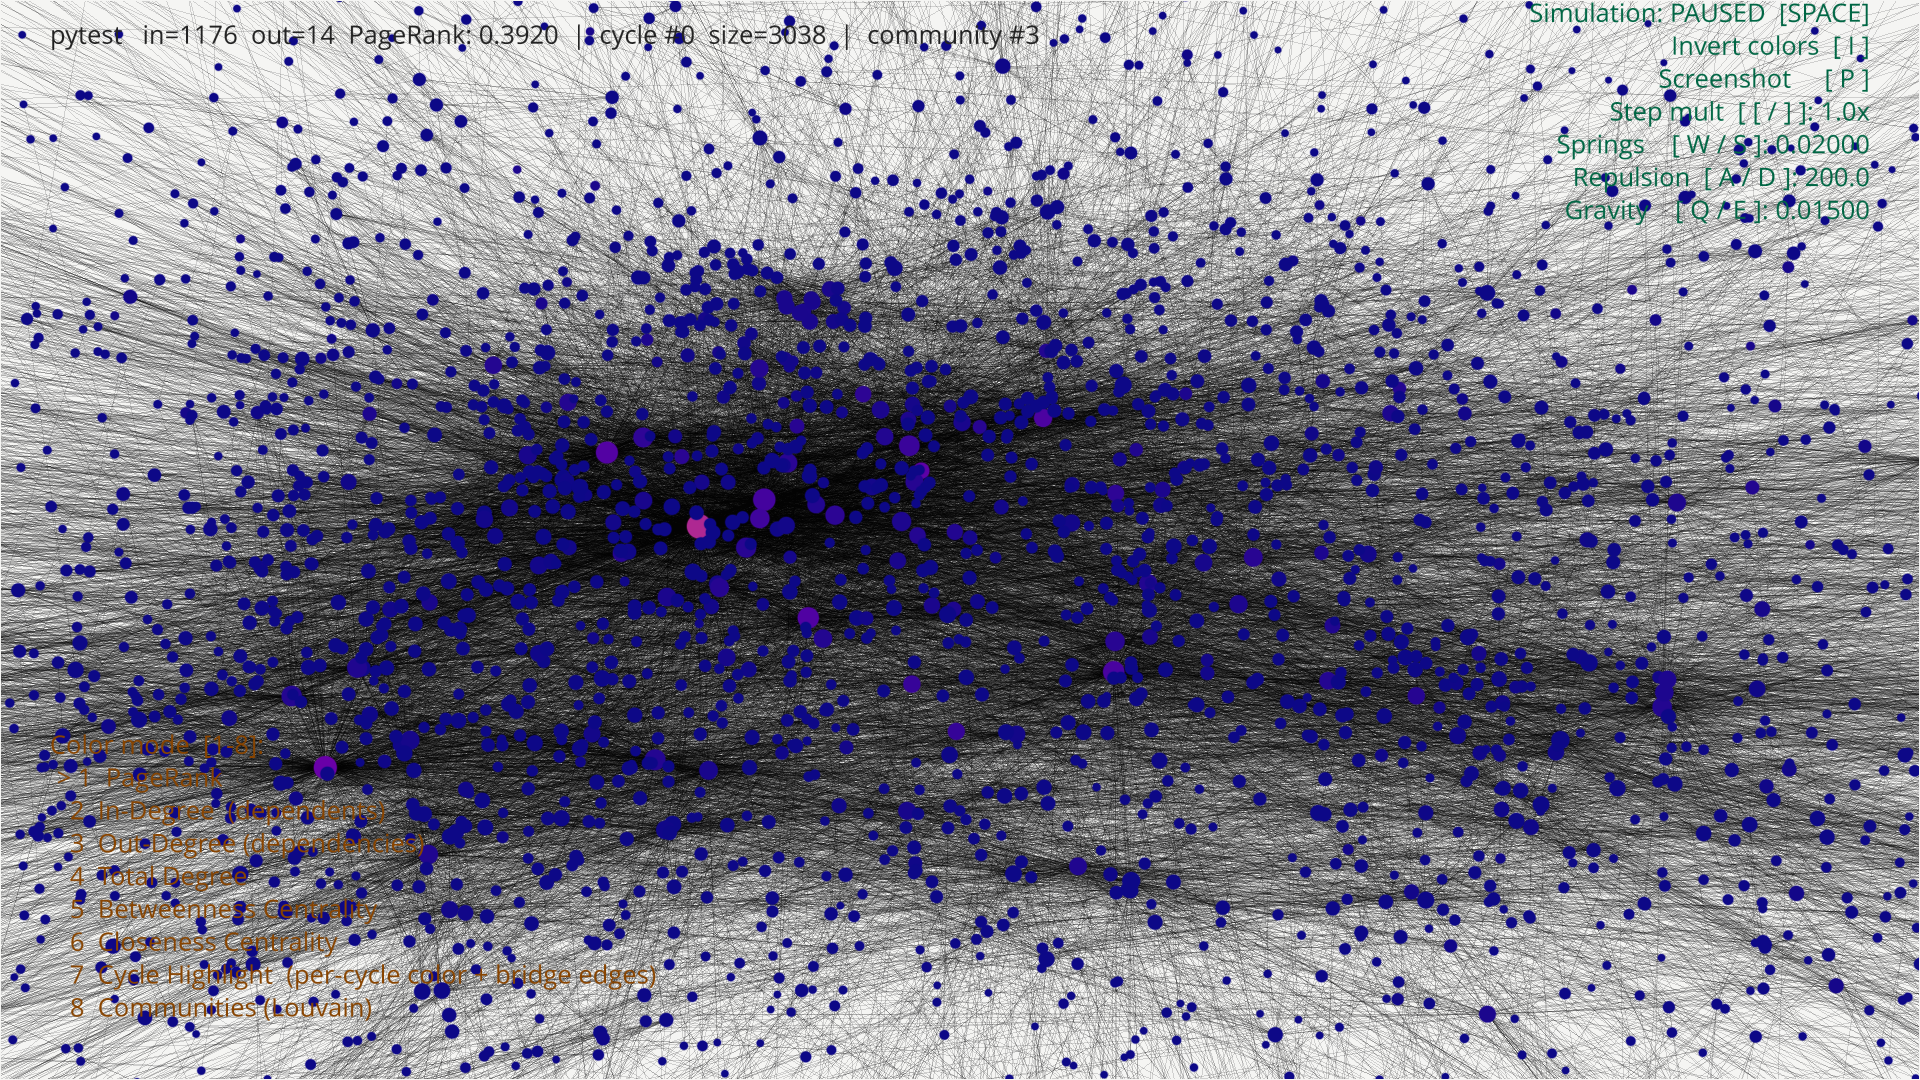
\includegraphics[width=1\linewidth]{Imagenes/PageRank_In}
		\caption{Representación del PageRank en la red con zoom de dependencias de Python donde en amarillo están los paquetes con mayor valor de esta métrica y en azul aquellos con menor valor.}
		\label{fig:pagerankin}
	\end{figure}
	
	Aun así, al analizar estos paquetes que han salido con los valores más elevados de este métrica de centralidad se confirma que esta es adecuada para el análisis de importancia pues los paquetes que salen arriba del todo son fundamentales. \texttt{typing-extensions} es una librería utilizada para forzar la definición explícita de los tipos de datos en Python. De esta manera, se soluciona el problema fundamental de los errores de tipo en el intérprete, lo que da sentido a que sea uno de los paquetes más relevantes del ecosistema. \texttt{pytest} el segundo de la lista es un paquete también esencial para el desarrollo porque es una herramienta necesaria en proyectos grandes para poder realizar los test del código. \texttt{numpy} es el tercero de la lista y es el paquete para realizar álgebra de manera eficiente en Python por lo que es lógico que tenga mucha relevancia porque la mayoría de paquetes necesitan realizar operaciones eficientes. Por tanto, el PageRank es una buena medida para evaluar como de útil es un paquete dentro del ecosistema de desarrollo.
	\newline
	
	Asimismo, es necesario recalcar el problema de la duplicidad de nodos introducido por cómo se ha construido el grafo. Tal y como se evidenció previamente con el paquete \texttt{ansible}, las inconsistencias en la nomenclatura utilizada por los desarrolladores provocan que una librería pueda no ser encontrada o crear entradas duplicadas. Esto implica que los paquetes más relevantes del ecosistema concentran, en realidad, un \textit{PageRank} aún mayor del que reflejan sus métricas individuales actuales. Ejemplos claros de esta división se observan en las entradas separadas para \texttt{typing-extensions} y \texttt{typing\_extensions}, o \texttt{sphinx} y \texttt{Sphinx}. Para resolver esta problemática, en PyPi probablemente se utilicen herramientas que conviertan todos los nombres a texto plano y de esta forma se eliminen estas inconsistencias.
	\newline
	
	Por otro lado, cabe destacar que, excluyendo a \texttt{numpy} y \texttt{requests} (que son paquetes de uso directo para aplicaciones muy específicas), la mayor parte del top 10 está conformada por paquetes necesarias para mantener proyectos complejos. En consecuencia, se evidencia que los paquetes más importantes de la red representan la infraestructura clave que permite al resto de herramientas tener un ciclo de desarrollo más ágil y escalable.
	\newline
	
	Finalmente, resulta llamativo encontrar en la quinta posición a \texttt{pyobjc-core}, una librería exclusiva para la integración con sistemas operativos macOS. Dado que el ecosistema de desarrollo en Python está fuertemente dominado por entornos Linux y Windows, la cuota de mercado de macOS no justificaría por sí sola una centralidad tan elevada. Sin embargo, esta anomalía ilustra perfectamente la naturaleza de las dependencias condicionales en proyectos multiplataforma. Grandes paquetes de automatización o interfaces gráficas incluyen a \texttt{pyobjc-core} como dependencia oculta, instalándose automáticamente solo cuando el código se ejecuta en un entorno de Apple. Así, la librería acumula un \textit{PageRank} masivo de forma pasiva.
	
	Por último, es relevante destacar como en el top 5 aparece el paquete \texttt{pyobjc-core} que es un paquete exclusivo para la integración con sistemas operativos macOS. Dado que la mayoría del desarrollo en Python está fuertemente dominado por entornos Linux y Windows, la cuota de mercado de macOS no justificaría por sí sola una centralidad tan elevada. No obstante, esta anomalía evidencia la naturaleza de las dependencias condicionales en proyectos multiplataforma que descargan este paquete solo cuando el código se ejecuta en entornos de Apple.
	
	\subsection{Centralidad de Intermediación}
	
	La centralidad de intermediación mide la frecuencia con la que un nodo esta en el camino más corto entre otros dos nodos del grafo. En el contexto del ecosistema Python, esta métrica indica que paquetes conectan paquetes de diferentes ecosistemas o que funcionan de interfaces estandarizadoras de los datos. Visualmente en las figuras \ref{fig:btweenessout} y \ref{fig:btweenesin}, se puede ver que a diferencia del PageRank existe una mayor homogeneidad en cuanto a esta métrica de centralidad, es decir, ya no existen tantos paquetes críticos. 
	\begin{figure}[H]
		\centering
		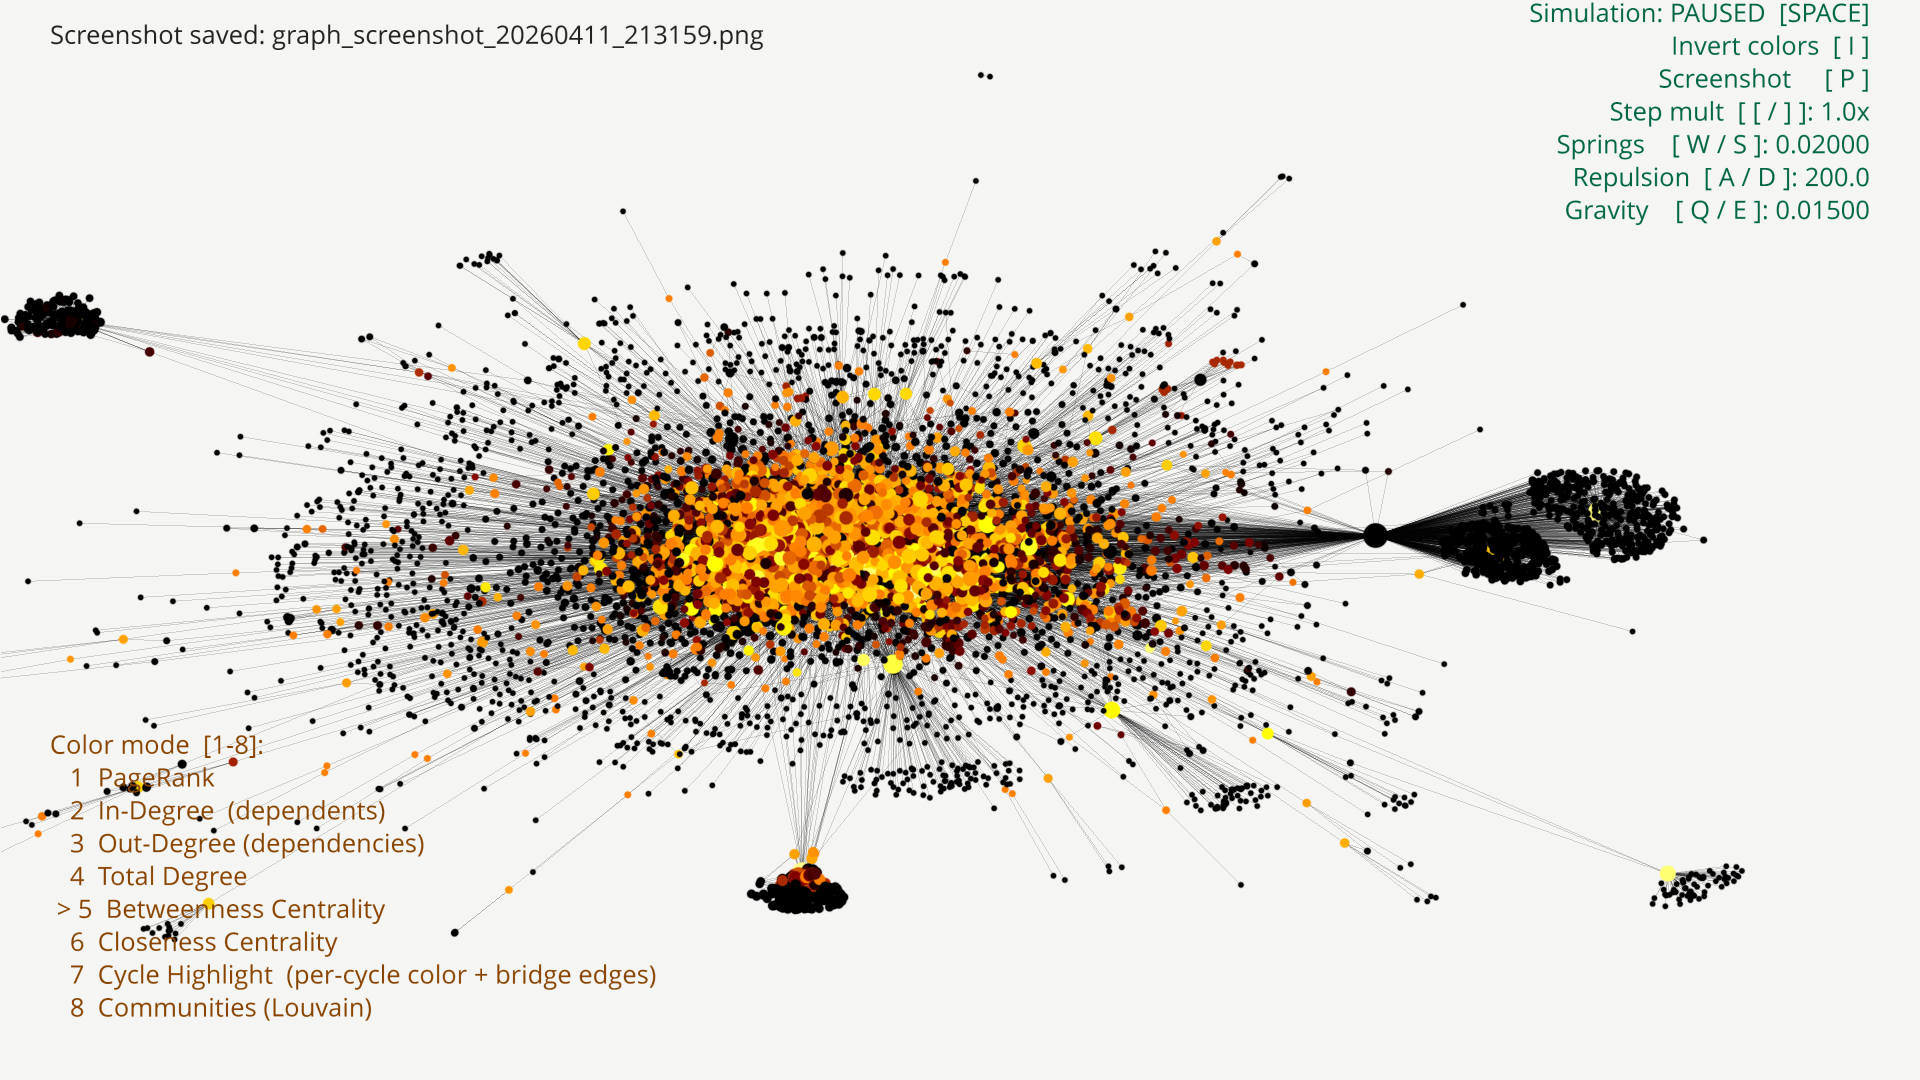
\includegraphics[width=1\linewidth]{Imagenes/BTWEENESSOUT}
		\caption{Representación de la Centralidad de Intermediación en la red completa de dependencias de Python donde en blanco y amarillo están los paquetes con mayor valor de esta métrica y en negro y rojo aquellos con menor valor.}
		\label{fig:btweenessout}
	\end{figure}
	\begin{figure}[H]
		\centering
		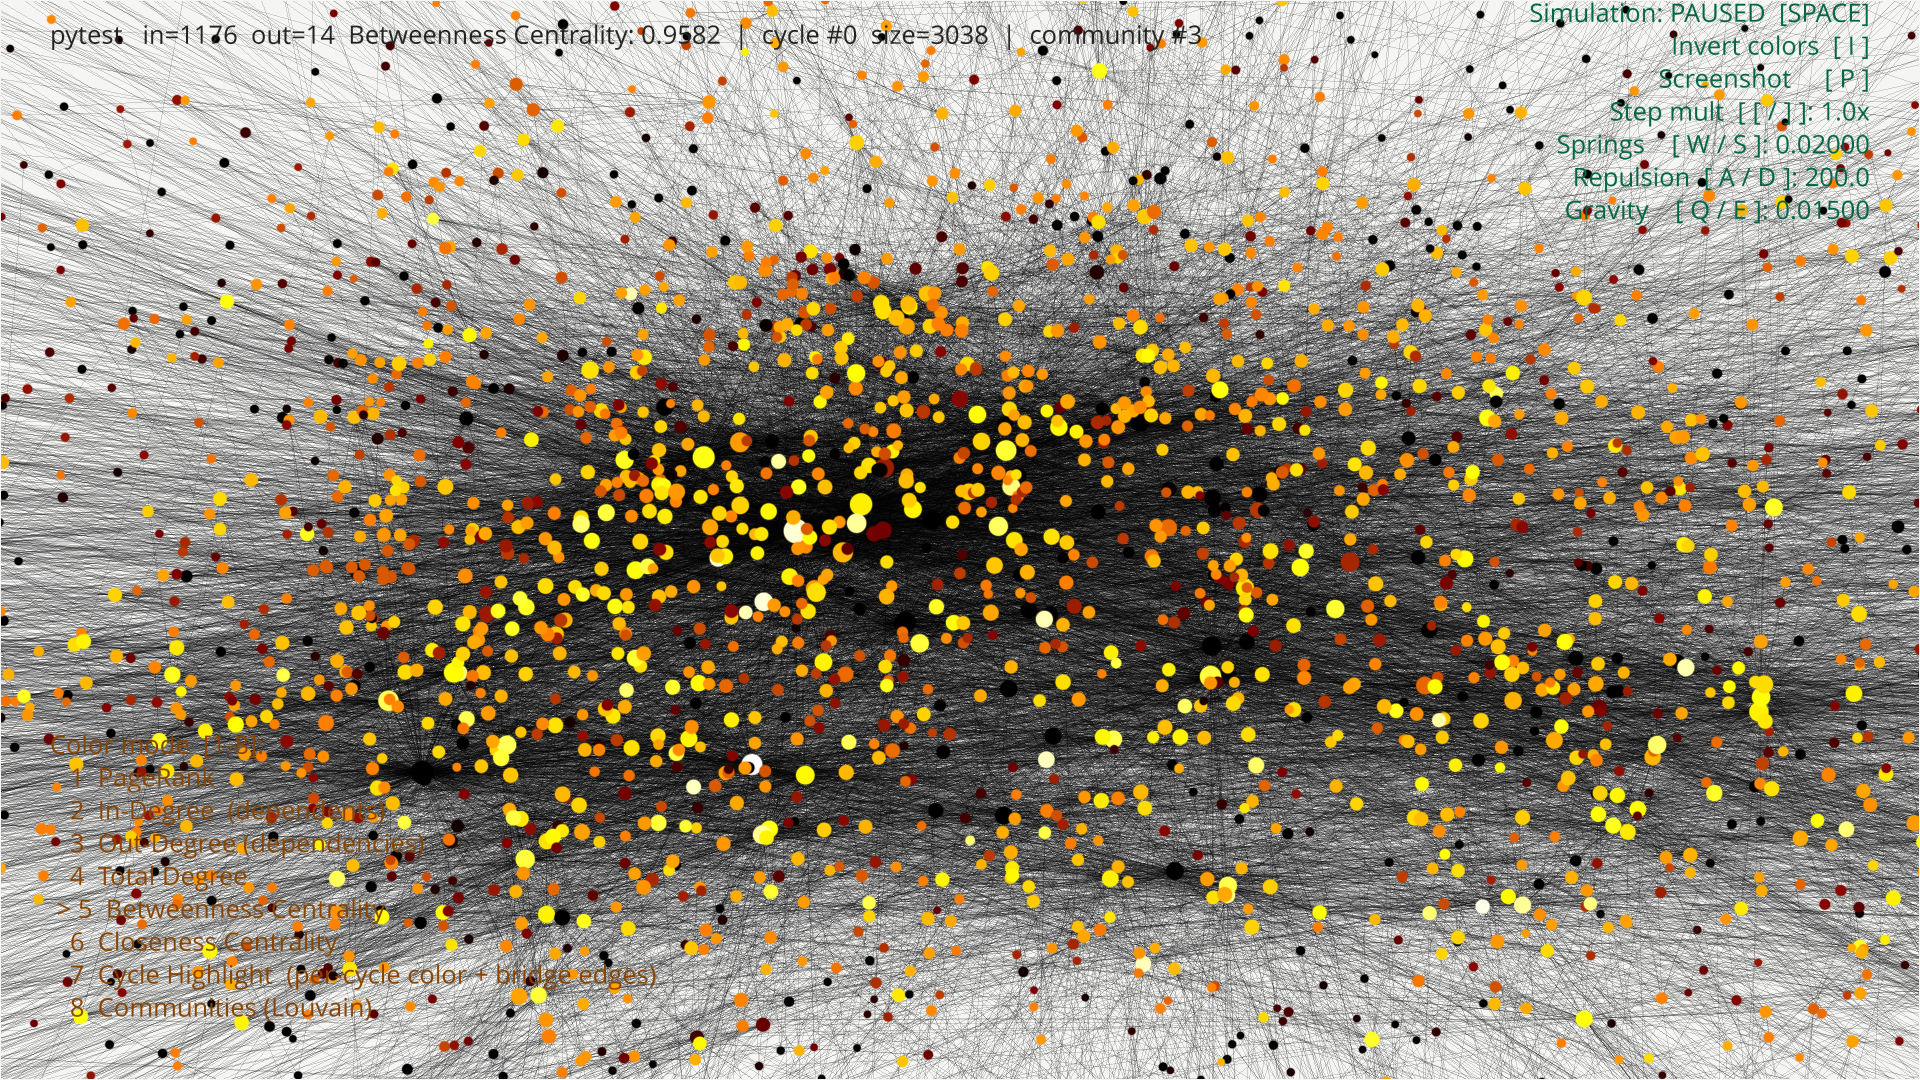
\includegraphics[width=1\linewidth]{Imagenes/BTWEENESIN}
		\caption{Representación de la Centralidad de Intermediación en la red con zoom de dependencias de Python donde en blanco y amarillo están los paquetes con mayor valor de esta métrica y en negro y rojo aquellos con menor valor.}
		\label{fig:btweenesin}
	\end{figure}
	
	Al examinar las primeras posiciones de esta métrica, se comprueba que refleja fielmente la función de estos paquetes como puentes del ecosistema. \texttt{pandas} ocupa el primer lugar al ser el estándar de facto para la manipulación de datos tabulares. Por tanto, su integración es un requisito para casi cualquier librería orientada al análisis de datos. A continuación, la segunda posición de \texttt{pyiceberg} subraya el inmenso peso que tiene el procesamiento de grandes volúmenes de información en Python en formato tabular. Dada su alta centralidad de intermediación, la adopción masiva de estas herramientas sugiere que la manipulación de datos tabulares es tan esencial dentro del ecosistema Python que podría motivar su futura integración como un tipo nativo en el estándar de Python.
	\newline
	
	A continuación, destaca la posición de \texttt{ipython}, que actúa como nexo fundamental entre los entornos de programación interactiva como Jupyter y las herramientas de depuración del lenguaje. Esta librería funciona como un puente estructural, conectando a la vasta comunidad centrada en el análisis exploratorio con el núcleo de desarrollo tradicional de Python. Por otro lado, la presencia de \texttt{hypothesis} y \texttt{pytest} cerrando el \textit{top} 5 revela la transversalidad de las pruebas de software. Independientemente del subdominio al que pertenezca un paquete, el uso de estos frameworks es un estándar para garantizar la calidad y compatibilidad del código, convirtiéndolos en puntos que unen todas las ramas de la red.

	\subsection{Centralidad de Cercania}

	La centralidad de cercanía evalúa la distancia media desde un nodo hacia todos los demás nodos de la red. Desde una perspectiva de arquitectura, esto implica que cualquier cambio en estos nodos centrales se propagará rápidamente a lo largo de toda la red.	Visualmente, tal y como se observa en las figuras \ref{fig:closenessout} y \ref{fig:closenessin}, la red presenta una apariencia densa y comprimida donde resulta complejo distinguir variaciones significativas entre los nodos Esta homogeneidad visual se debe a la componente no conexa del paquete \texttt{ansible} que provoca una distorsión que aplasta los valores de centralidad de la inmensa mayoría de la red principal en torno al $0.4$. Para mitigar este efecto y poder extraer conclusiones analíticas válidas este paquete se ha sido excluido del ranking numérico analizado a continuación.
	
	
	\begin{figure}[H]
		\centering
		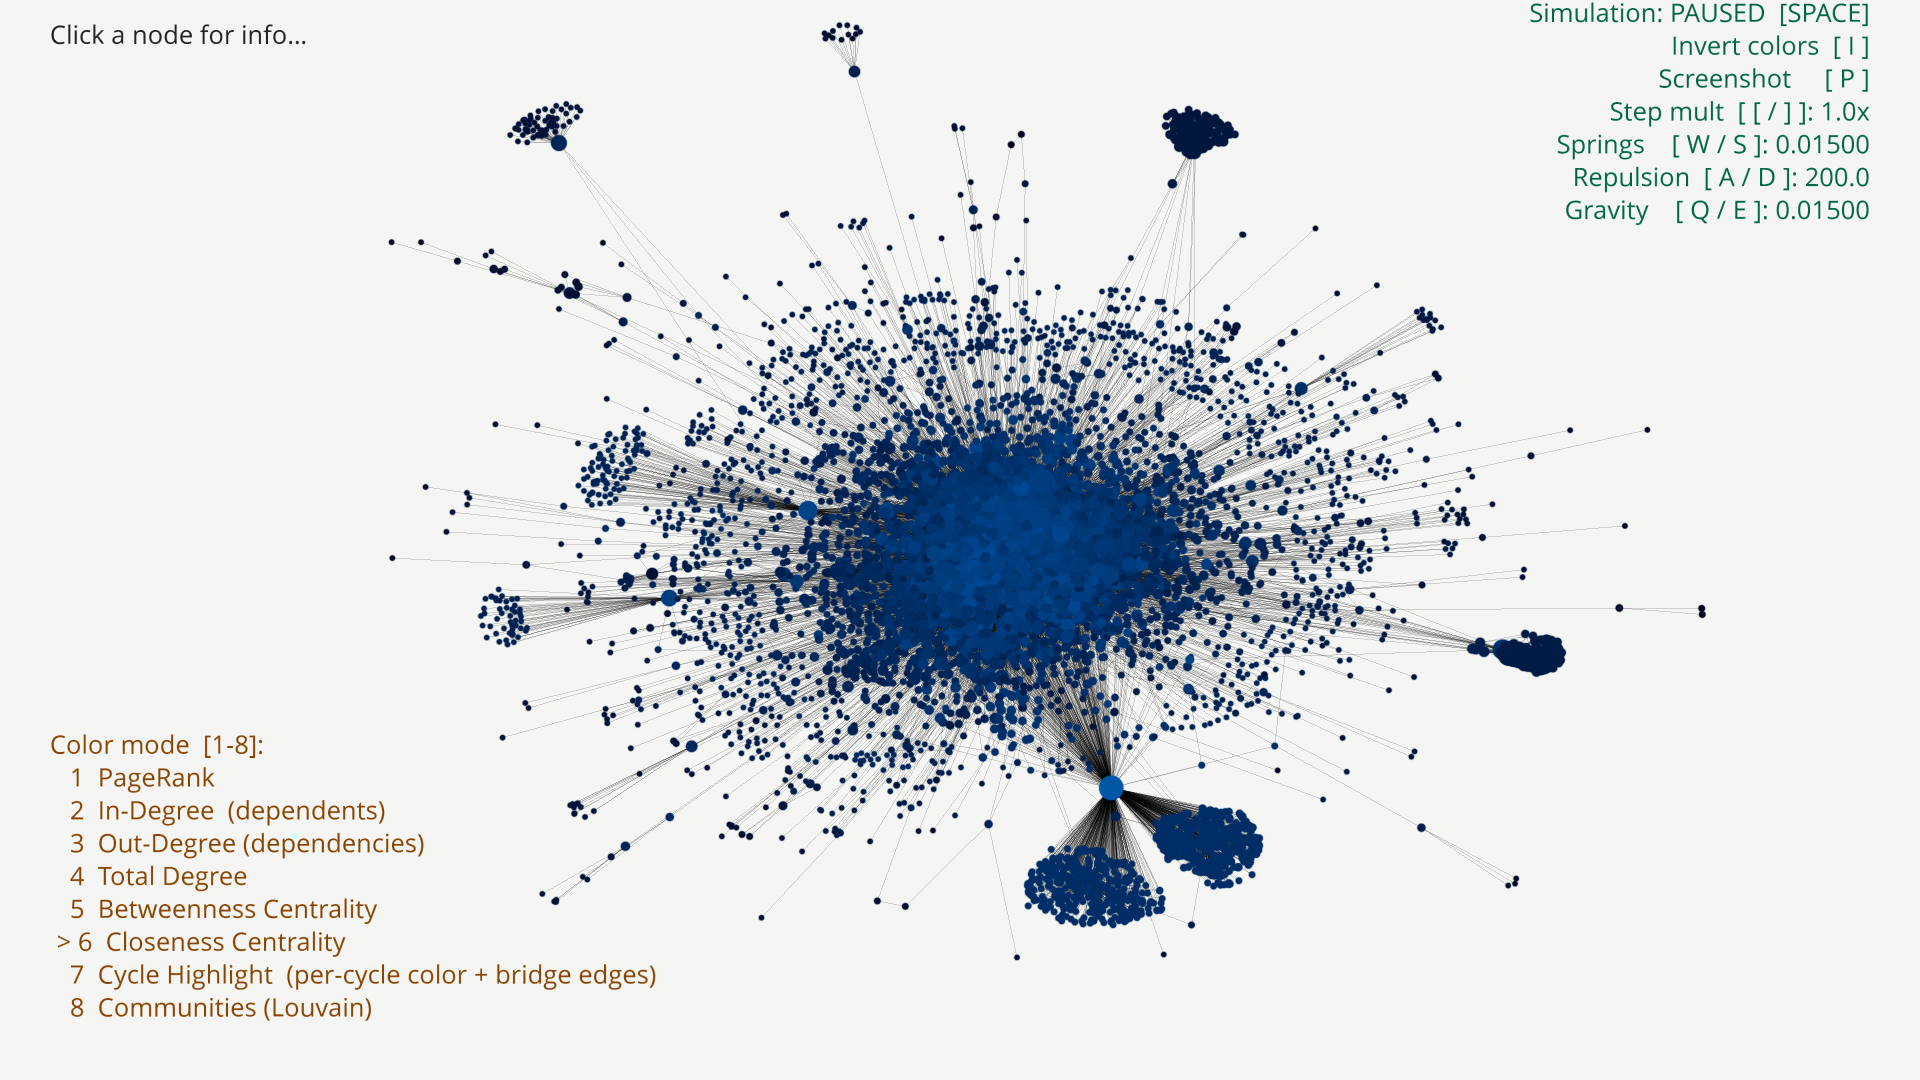
\includegraphics[width=1\linewidth]{Imagenes/Closeness_Out}
		\caption{Representación de la Centralidad de Cercanía en la red completa de dependencias de Python donde en blanco y cian están los paquetes con mayor valor de esta métrica y en azul oscuro aquellos con menor valor.}
		\label{fig:closenessout}
	\end{figure}
	
	\begin{figure}[H]
		\centering
		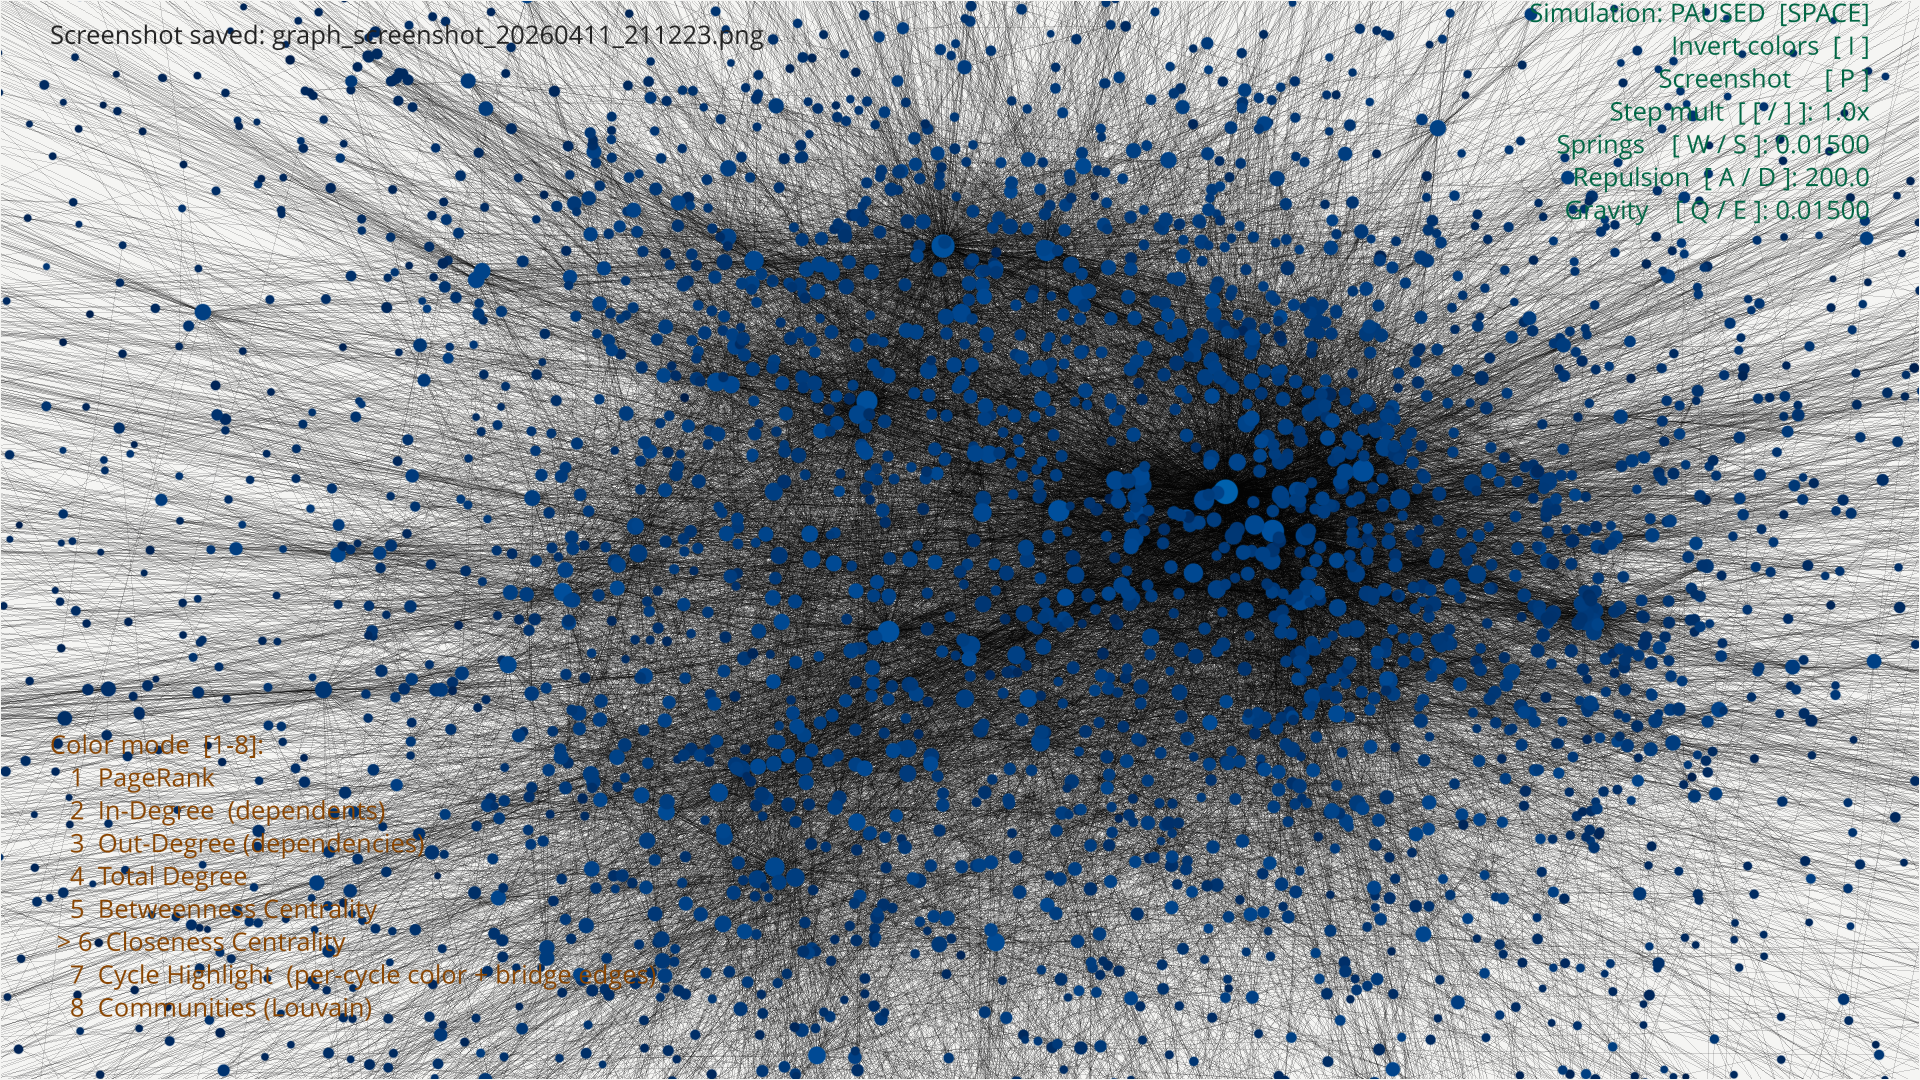
\includegraphics[width=1\linewidth]{Imagenes/Closeness_In}
		\caption{Representación de la Centralidad de Cercanía en la red con zoom de dependencias de Python donde en blanco y cian están los paquetes con mayor valor de esta métrica y en azul oscuro aquellos con menor valor.}
		\label{fig:closenessin}
	\end{figure}

	
Al examinar los datos depurados y normalizados, no se observan grandes diferencias entre los paquetes y parecen estar distribuidos de manera muy uniforme. No obstante, las conclusiones de centralidad que se obtienen son semejantes a las obtenidas mediante las métricas de PageRank y de centralidad de intermediación.

\subsection{Distribuciones de Centralidad}

Para comprender la topología de la red de dependencias, es fundamental analizar la distribución de sus métricas de centralidad. Al observar las figuras \ref{fig:centralitydistributionslinear} y \ref{fig:centralitydistributionsloglog}, se identifican tres patrones geométricos distintos que responden a leyes matemáticas específicas.

\begin{figure}[H]
	\centering
	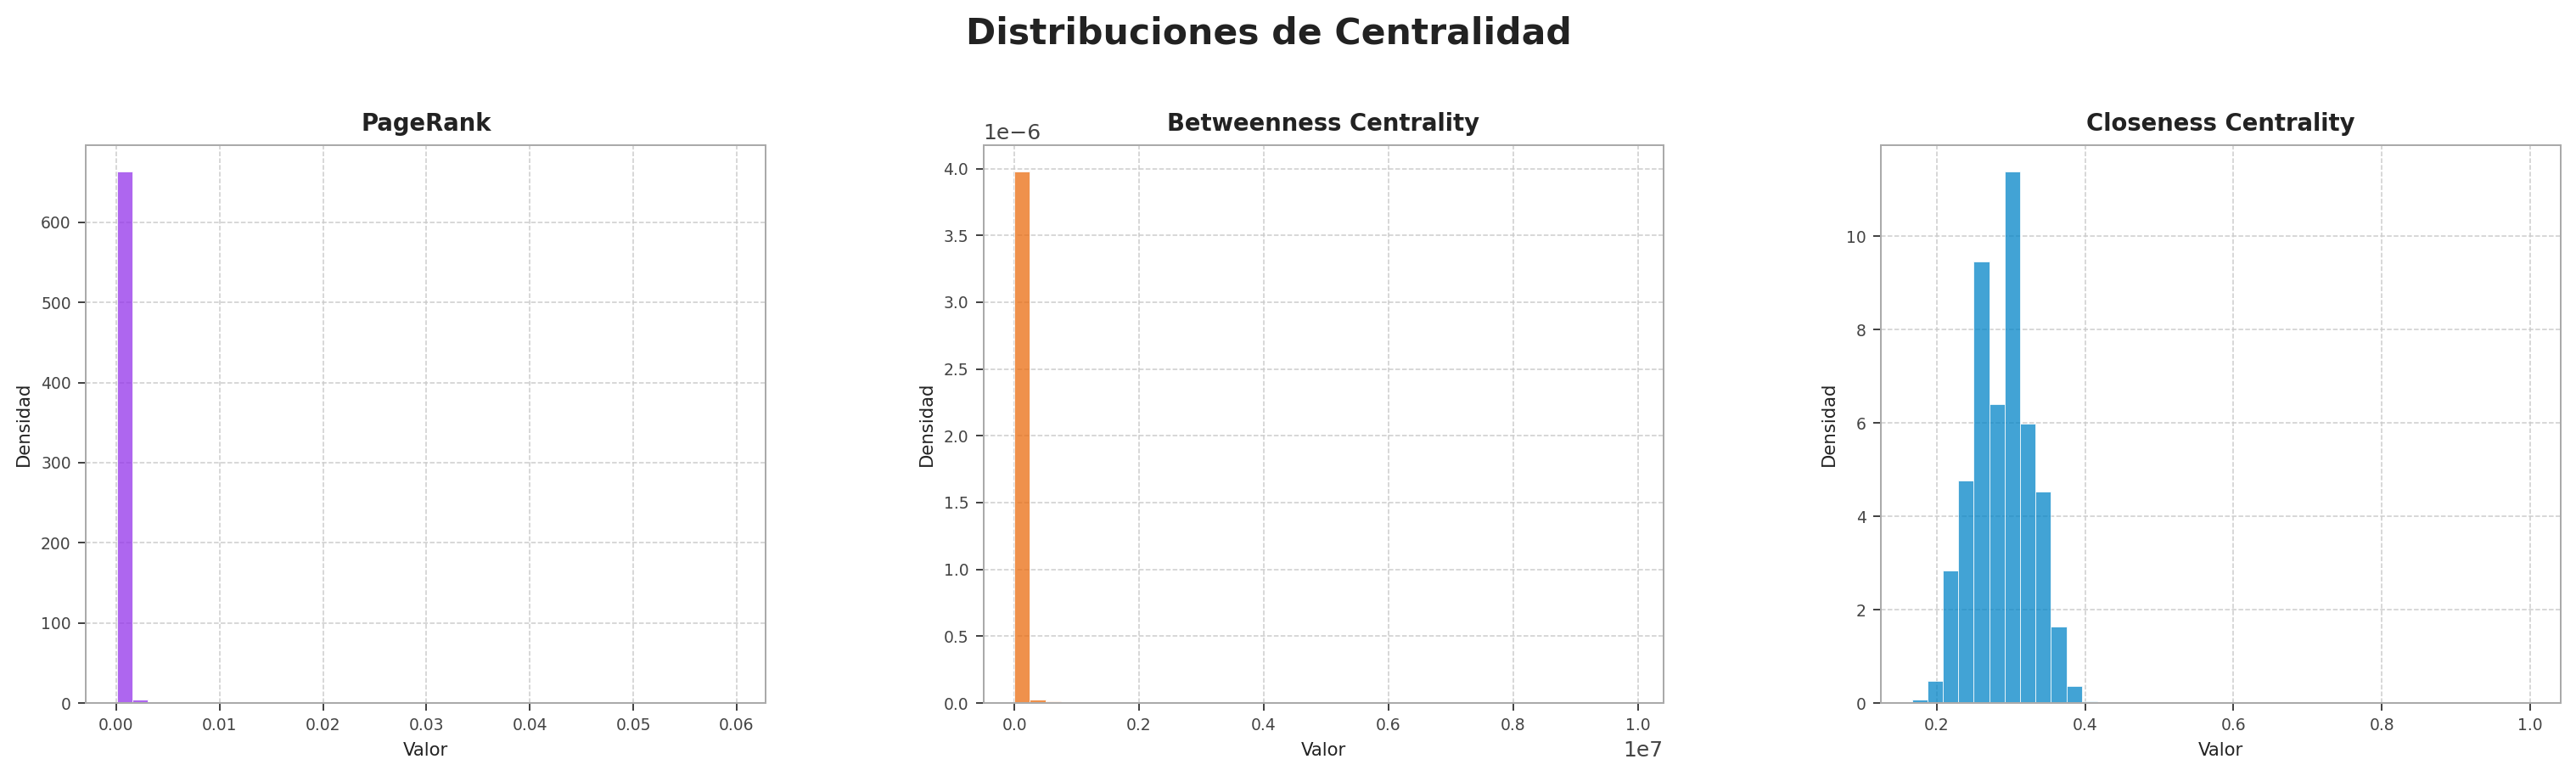
\includegraphics[width=1\linewidth]{Imagenes/centrality_distributions_linear}
	\caption{Distribución de frecuencias de las métricas de centralidad en escala lineal. Se observa una asimetría extrema en la mayoría de variables.}
	\label{fig:centralitydistributionslinear}
\end{figure}

\begin{figure}[H]
	\centering
	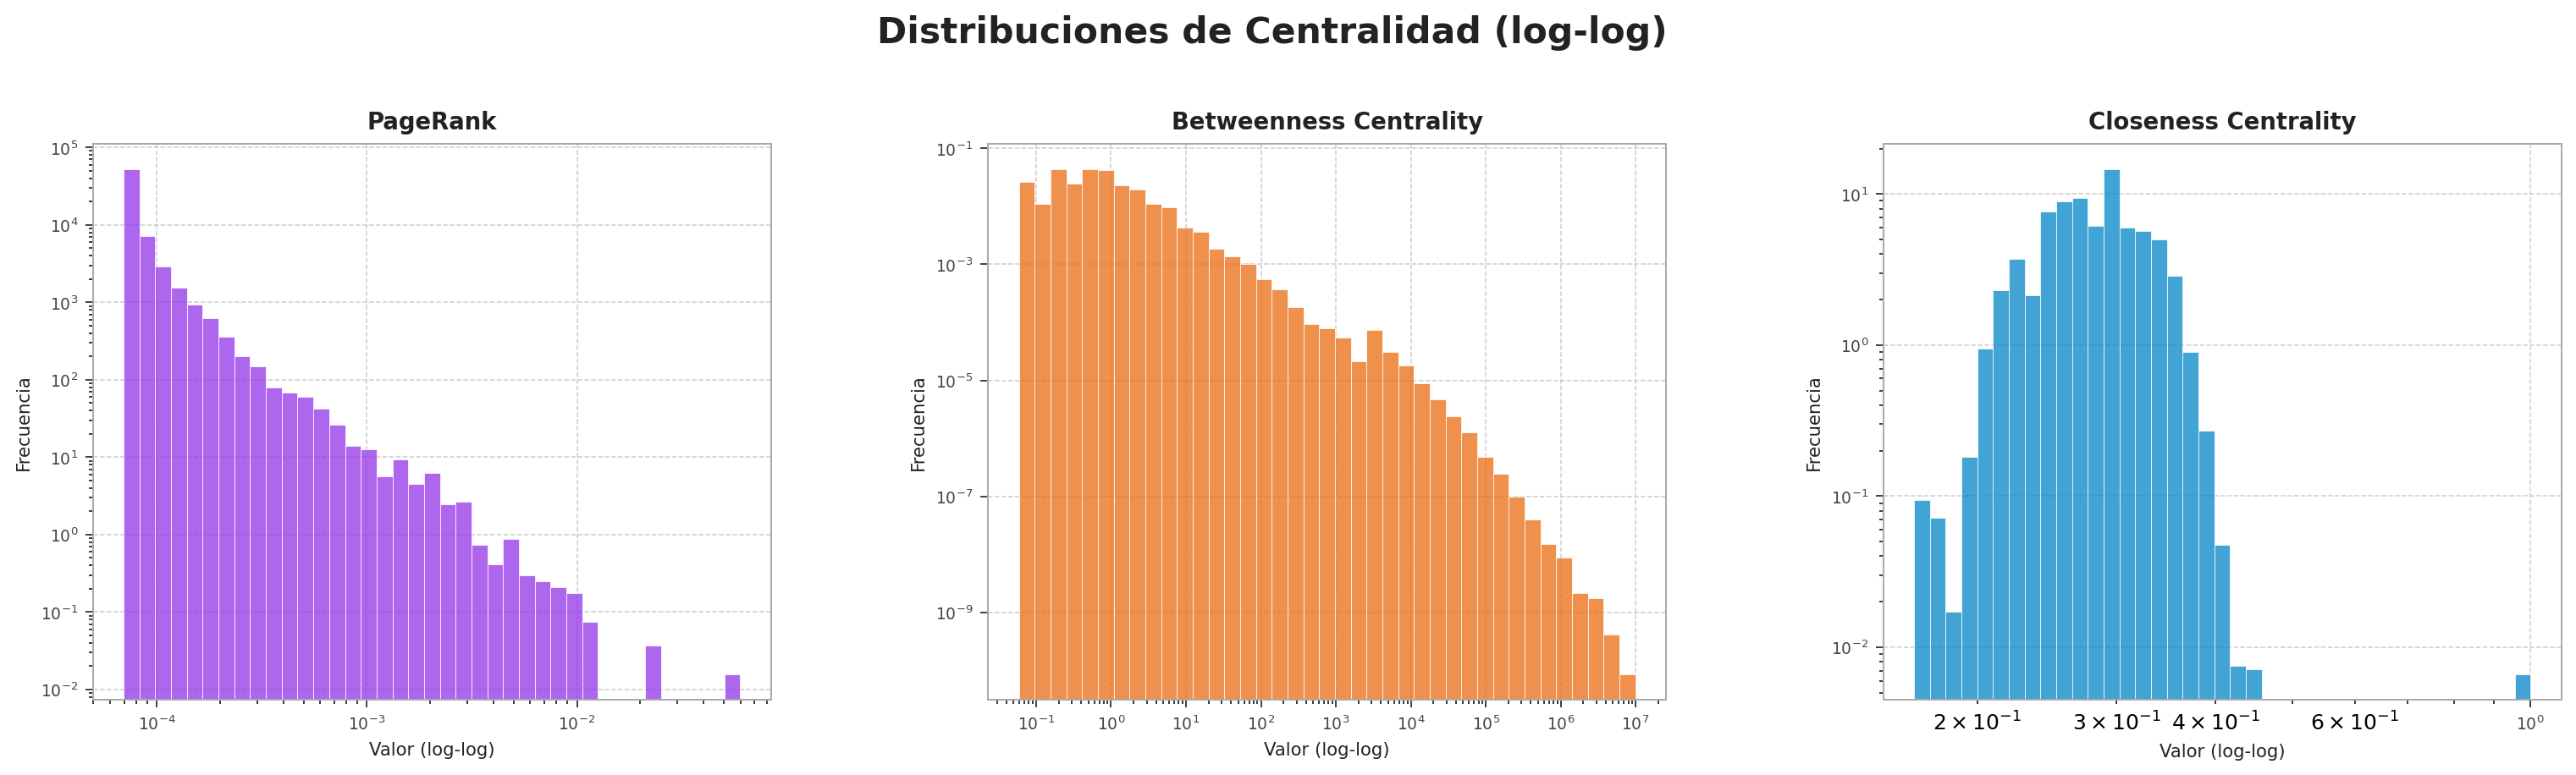
\includegraphics[width=1\linewidth]{Imagenes/centrality_distributions_loglog}
	\caption{Distribución de frecuencias de las métricas de centralidad en escala Log-Log, revelando las leyes de potencias y decaimientos estructurales.}
	\label{fig:centralitydistributionsloglog}
\end{figure}

\subsubsection{PageRank}
En la escala Log-Log, esta métrica se distribuye siguiendo una línea recta descendente. Este comportamiento es característico de las redes libres de escala, donde la función sigue la relación:
\begin{equation}
	P(PR) \sim PR^{-\gamma} \implies \log(P(PR)) = -\gamma \log(PR) + C
\end{equation}

Este comportamiento muestra que los paquetes más importantes siguen creciendo y siendo cada vez más importantes, es decir, un escenario de rich get richer. Dentro de un ecosistema de paquetes esto es lógico puesto que existen dependencias que por la función esencial que desempeñan acaban siendo los más importantes.


\subsubsection{Centralidad de Intermediación}
A diferencia de la anterior, la centralidad de intermediación no forma una recta, sino una curva que cae de forma cuadrática en la escala logarítmica. Esta relación tiene una ecuación de tipo:
\begin{equation}
	\log(P(CI)) \approx -K (\log CI)^2 + C
\end{equation}
Esta curvatura indica que ser un puente es un rol mucho más exclusivo que ser popular.
\subsubsection{Centralidad de Cercanía}
La centralidad de cercanía rompe con las asimetrías anteriores y presenta una distribución similar a una distribución normal:
\begin{equation}
	P(CC) = \frac{1}{\sigma\sqrt{2\pi}} e^{-\frac{1}{2}\left(\frac{CC-\mu}{\sigma}\right)^2}
\end{equation}
Este fenómeno se debe a la existencia del efecto Pequeño Mundo. 
	\section{Análisis de comunidades}
Para analizar las comunidades se utiliza el algoritmo de Louvain aplicado sobre el grado no dirigido. El análisis de esta sección queda reflejado mediante la figuras \ref{fig:comunidades}, \ref{fig:communitiesdonut} y la tabla \ref{tab:communities_desc} generada mediante el script \texttt{comunities.py}. ITS NOT WORKING PROPERLY CHECK RNG; REDO TABLE AND PNG
\begin{figure}[H]
	\centering
	
\includegraphics[width=1\linewidth]{Imagenes/Comunidades}
	\caption{}
	\label{fig:comunidades}
\end{figure}


\renewcommand{\arraystretch}{1.5}
\begin{longtable}{|c|c|p{10cm}|}
	\caption{Descripción de las comunidades principales detectadas en la red de dependencias de Python.} \label{tab:communities_desc} \\
	
	\hline
	\textbf{ID} & \textbf{Nodos} & \textbf{Descripción} \\ \hline
	\endhead
	
	\hline
	\multicolumn{3}{|r|}{{Continúa en la siguiente página...}} \\ \hline
	\endfoot
	
	\hline
	\endlastfoot
	
	\cellcolor[RGB]{235,59,59}0 & 413 &  Ecosistema orientado a computación interactiva y documentación científica (\texttt{jupyter}, \texttt{jupyterlab}, \texttt{notebook}). Destaca una infraestructura completa de kernels y servidores Jupyter (\texttt{ipykernel}, \texttt{jupyter-server}, \texttt{jupyter-client}), acompañada de un ecosistema de widgets e interfaces enriquecidas (\texttt{ipywidgets}, \texttt{ipyvuetify}, \texttt{ipyleaflet}, \texttt{ipympl}). Se complementa con herramientas de documentación técnica y generación de sitios estáticos basados en Sphinx (\texttt{sphinx-design}, \texttt{pydata-sphinx-theme}, \texttt{nbsphinx}, \texttt{myst-parser}), junto a utilidades de testing y validación de notebooks (\texttt{nbval}, \texttt{nbmake}, \texttt{pytest-jupyter}).\\ \hline
	\cellcolor[RGB]{235,98,59}1 & 1197 & Ecosistema moderno de desarrollo web asíncrono y APIs (\texttt{fastapi}, \texttt{starlette}, \texttt{pydantic}, \texttt{uvicorn}), con soporte completo para autenticación y seguridad (\texttt{cryptography}, \texttt{pyjwt}, \texttt{authlib}, \texttt{bcrypt}). Destaca una integración masiva con infraestructura para IA Generativa y LLMs (\texttt{openai}, \texttt{anthropic}, \texttt{langchain}, \texttt{llama-index}, \texttt{pydantic-ai}, \texttt{litellm}), apoyada por clientes de red asíncronos (\texttt{httpx}, \texttt{aiohttp}) y herramientas de observabilidad y telemetría (\texttt{opentelemetry-api}, \texttt{opentelemetry-sdk}, \texttt{logfire}, \texttt{sentry-sdk}). Se complementa con conectores a múltiples bases de datos y servicios cloud (\texttt{pymongo}, \texttt{redis}, \texttt{sqlalchemy}, \texttt{boto3}, \texttt{azure-core}), orquestación de agentes y flujos de trabajo (\texttt{langgraph}, \texttt{celery}, \texttt{prefect}, \texttt{ray}) y soporte para el protocolo MCP (\texttt{mcp}, \texttt{fastmcp}). \\ \hline
	\cellcolor[RGB]{235,137,59}2 & 867 & Ecosistema dominado casi en su totalidad por definiciones de tipos estáticos para AWS (\texttt{types-boto3}, \texttt{types-aiobotocore}), cubriendo de forma exhaustiva la práctica totalidad de servicios de la nube de Amazon, tanto en su variante síncrona como asíncrona. Más allá de las anotaciones de tipo, se observan utilidades de análisis estático y herramientas de datos de alto rendimiento (\texttt{polars}, \texttt{blake3}, \texttt{pyzstd}), junto a componentes auxiliares de serialización y reflexión de tipos (\texttt{databind.core}, \texttt{databind.json}, \texttt{typeapi}). \\ \hline
	\cellcolor[RGB]{235,176,59}3 & 641 &  Ecosistema centrado en análisis y manipulación de datos tabulares y científicos (\texttt{pandas}, \texttt{polars}, \texttt{dask}, \texttt{xarray}, \texttt{numpy}), con soporte extenso para formatos de archivo y serialización (\texttt{pyarrow}, \texttt{fastparquet}, \texttt{openpyxl}, \texttt{pyiceberg}, \texttt{fastavro}). Destaca una infraestructura amplia de conectividad con bases de datos relacionales y analíticas (\texttt{sqlalchemy}, \texttt{duckdb}, \texttt{psycopg2}, \texttt{connectorx}, \texttt{clickhouse-connect}), junto a herramientas de computación distribuida y procesamiento a escala (\texttt{pyspark}, \texttt{ray}, \texttt{datafusion}, \texttt{modin}). Se complementa con un ecosistema de visualización y geoespacial (\texttt{plotly}, \texttt{bokeh}, \texttt{geopandas}, \texttt{cartopy}, \texttt{folium}) y librerías científicas de dominio específico (\texttt{astropy}, \texttt{stumpy}, \texttt{statsmodels}).\\ \hline
	\cellcolor[RGB]{235,215,59}4 & 1128 & Ecosistema orientado al desarrollo, empaquetado y control de calidad de software Python (\texttt{setuptools}, \texttt{flit}, \texttt{hatchling}, \texttt{build}, \texttt{twine}). Destaca una infraestructura muy extensa de testing y cobertura (\texttt{pytest}, \texttt{pytest-cov}, \texttt{pytest-mock}, \texttt{pytest-benchmark}, \texttt{tox}), acompañada de un conjunto exhaustivo de herramientas de análisis estático, linting y formateo (\texttt{mypy}, \texttt{flake8}, \texttt{pylint}, \texttt{black}, \texttt{isort}, \texttt{ruff}). Se complementa con generación de documentación técnica basada en Sphinx (\texttt{sphinx}, \texttt{sphinx-rtd-theme}, \texttt{sphinxcontrib-*}), junto a frameworks de GUI e interfaces de escritorio (\texttt{kivy}, \texttt{qtpy}) y herramientas de empaquetado y distribución de aplicaciones (\texttt{pyinstaller}, \texttt{nuitka}, \texttt{cibuildwheel}). \\ \hline
	\cellcolor[RGB]{215,235,59}5 & 1169 & Ecosistema orientado al aprendizaje automático profundo y la computación científica de alto rendimiento, articulado en torno a los principales frameworks de deep learning (\texttt{tensorflow}, \texttt{torch}, \texttt{jax}, \texttt{keras}, \texttt{flax}, \texttt{mxnet}). Incorpora una infraestructura GPU muy extensa basada en bibliotecas NVIDIA (\texttt{nvidia-cublas-cu12}, \texttt{nvidia-cudnn-cu12}, \texttt{nvidia-cuda-nvcc-cu12}, \texttt{triton}) junto a aceleradores de inferencia y optimización de modelos (\texttt{onnxruntime}, \texttt{vllm}, \texttt{deepspeed}, \texttt{bitsandbytes}, \texttt{optimum}, \texttt{torch-tensorrt}). Destaca un completo stack de procesamiento del lenguaje natural y modelos generativos (\texttt{transformers}, \texttt{tokenizers}, \texttt{sentence-transformers}, \texttt{huggingface-hub}, \texttt{peft}, \texttt{trl}, \texttt{diffusers}, \texttt{accelerate}), acompañado de soporte para visión artificial (\texttt{torchvision}, \texttt{opencv-python}, \texttt{Pillow}, \texttt{kornia}, \texttt{timm}, \texttt{albumentations}) y procesamiento de audio (\texttt{librosa}, \texttt{soundfile}, \texttt{torchaudio}). Se complementa con herramientas de computación científica de propósito general (\texttt{numpy}, \texttt{scipy}, \texttt{matplotlib}, \texttt{scikit-learn}, \texttt{statsmodels}), gestión de datos a escala (\texttt{datasets}, \texttt{dask}, \texttt{fsspec}) y aprendizaje por refuerzo (\texttt{gymnasium}, \texttt{ray}, \texttt{mujoco}, \texttt{brax}). \\ \hline
	\cellcolor[RGB]{176,235,59}6 & 179 & Ecosistema centrado en la aceleración GPU mediante CUDA y el stack RAPIDS para computación analítica a escala, articulado en torno a las interfaces de bajo nivel de CUDA (\texttt{cuda-bindings}, \texttt{cuda-python}, \texttt{cuda-core}, \texttt{cuda-toolkit}) y las bibliotecas de álgebra lineal y procesamiento masivo en GPU (\texttt{cupy}, \texttt{numba-cuda}, \texttt{nvidia-cudnn-frontend}, \texttt{nvidia-cutlass-dsl}). Incorpora el ecosistema RAPIDS completo para análisis de datos sobre GPU (\texttt{cudf}, \texttt{pylibcudf}, \texttt{rmm}, \texttt{kvikio}, \texttt{dask-cuda}, \texttt{dask-cudf}, \texttt{rapidsmpf}), junto a soporte de imagen y compresión acelerada (\texttt{nvidia-nvimgcodec-cu12}, \texttt{nvidia-nvjpeg-cu12}, \texttt{nvidia-libnvcomp}). Destaca una infraestructura de testing y garantía de calidad muy consolidada (\texttt{hypothesis}, \texttt{hypothesis-crosshair}, \texttt{dpcontracts}, \texttt{fixtures}, \texttt{testtools}, \texttt{stestr}, \texttt{codecov}), acompañada de herramientas de análisis estático y seguridad (\texttt{bandit}, \texttt{autopep8}, \texttt{pycodestyle}, \texttt{pydocstyle}, \texttt{pyupgrade}). Se incluye el stack completo de procesamiento del lenguaje natural de spaCy (\texttt{spacy}, \texttt{thinc}, \texttt{blis}, \texttt{preshed}, \texttt{srsly}, \texttt{weasel}) con soporte multilingüe extendido (\texttt{sudachipy}, \texttt{natto-py}, \texttt{ufal.udpipe}), una infraestructura de herramientas CLI orientada a OpenStack (\texttt{cliff}, \texttt{oslo.config}, \texttt{oslo.utils}, \texttt{pbr}, \texttt{stevedore}, \texttt{reno}) y utilidades de computación numérica de alta precisión (\texttt{mpmath}, \texttt{python-gmp}, \texttt{Cython}, \texttt{pyarrow}, \texttt{pandas}). \\ \hline
	\cellcolor[RGB]{137,235,59}7 & 157 &  Ecosistema centrado en la integración con la nube de Google y la comunicación entre servicios mediante gRPC y Protocol Buffers, articulado en torno a las bibliotecas principales de Google Cloud (\texttt{google-api-core}, \texttt{google-auth}, \texttt{google-cloud-core}, \texttt{proto-plus}, \texttt{protobuf}, \texttt{grpcio}). Cubre un amplio abanico de servicios gestionados de GCP, incluyendo almacenamiento y bases de datos (\texttt{google-cloud-storage}, \texttt{google-cloud-bigquery}, \texttt{google-cloud-bigtable}, \texttt{google-cloud-spanner}, \texttt{google-cloud-firestore}, \texttt{google-cloud-datastore}), mensajería y streaming (\texttt{google-cloud-pubsub}, \texttt{google-cloud-pubsublite}), seguridad y gestión de secretos (\texttt{google-cloud-kms}, \texttt{google-cloud-secret-manager}, \texttt{google-cloud-dlp}, \texttt{tink}), e inteligencia artificial aplicada (\texttt{google-cloud-vision}, \texttt{google-cloud-language}, \texttt{google-cloud-speech}, \texttt{google-generativeai}, \texttt{google-cloud-videointelligence}). Incorpora infraestructura para pipelines de MLOps y procesamiento a escala (\texttt{kfp}, \texttt{apache-beam}, \texttt{google-cloud-dataproc}, \texttt{tensorflow-serving-api}, \texttt{torchx}), junto a herramientas de autenticación y autorización OAuth (\texttt{google-auth-httplib2}, \texttt{oauth2client}, \texttt{pyasn1}, \texttt{rsa}, \texttt{pyu2f}). Se complementa con utilidades de testing orientadas a entornos cloud (\texttt{google-cloud-testutils}, \texttt{testcontainers}, \texttt{aioresponses}, \texttt{testslide}), análisis estático y refactorización de código (\texttt{libcst}, \texttt{pyannotate}, \texttt{mypy-extensions}, \texttt{pyre-check}) y herramientas de búsqueda vectorial y bases de datos externas (\texttt{google-cloud-vectorsearch}, \texttt{pinecone}, \texttt{opensearch-protobufs}).\\ \hline
	\cellcolor[RGB]{98,235,59}8 & 2 & Componente no conexa con ansible. \\ \hline
	\cellcolor[RGB]{59,235,59}9 & 205 &  Ecosistema orientado a la documentación técnica moderna y la orquestación de pipelines de datos, articulado en torno a MkDocs como plataforma principal de generación de documentación (\texttt{mkdocs}, \texttt{mkdocs-material}, \texttt{mkdocstrings}, \texttt{mkdocs-jupyter}, \texttt{mkdocs-gen-files}, \texttt{mkdocs-literate-nav}) con un extenso catálogo de plugins y extensiones asociadas (\texttt{mkdocs-redirects}, \texttt{mkdocs-minify-plugin}, \texttt{mkdocs-macros-plugin}, \texttt{mkdocs-rss-plugin}, \texttt{mkdocs-glightbox}, \texttt{pymdown-extensions}). Incorpora el framework Kedro para la construcción de pipelines de datos reproducibles y mantenibles (\texttt{kedro}, \texttt{kedro-datasets}), con conectores para una amplísima variedad de formatos y backends de almacenamiento incluyendo Spark y Delta Lake (\texttt{kedro-datasets[spark-]}, \texttt{kedro-datasets[delta-]}), bases de datos vectoriales (\texttt{kedro-datasets[chromadb-]}), modelos de lenguaje (\texttt{kedro-datasets[langchain-]}, \texttt{kedro-datasets[langfuse-]}) y formatos tabulares (\texttt{kedro-datasets[pandas-]}, \texttt{kedro-datasets[polars-*]}). Destaca el framework de consulta analítica Ibis con soporte para múltiples backends (\texttt{ibis-framework[duckdb]}, \texttt{ibis-framework[bigquery]}, \texttt{ibis-framework[postgres]}, \texttt{ibis-framework[pyspark]}, \texttt{ibis-framework[snowflake]}), junto a herramientas de computación tensorial dispersa (\texttt{sparse}, \texttt{zarr}, \texttt{numcodecs}, \texttt{finch-mlir}) y bibliotecas de deep learning funcional basadas en JAX (\texttt{equinox}, \texttt{jaxtyping}). Se complementa con utilidades de series temporales (\texttt{u8darts-all}), optimización de hiperparámetros (\texttt{ConfigSpace}) y herramientas auxiliares de testing y validación de proyectos (\texttt{pytest-cases}, \texttt{validate-pyproject}, \texttt{pytest-accept}).\\ \hline
	\cellcolor[RGB]{59,235,98}10 & 46 &  Ecosistema centrado en la transformación y orquestación de datos analíticos mediante dbt y Prefect, articulado en torno al núcleo de dbt (\texttt{dbt-core}, \texttt{dbt-common}, \texttt{dbt-adapters}, \texttt{dbt-protos}) con adaptadores para los principales data warehouses en la nube (\texttt{dbt-bigquery}, \texttt{dbt-snowflake}, \texttt{dbt-postgres}, \texttt{dbt-singlestore}). Incorpora el stack de orquestación de Prefect con integraciones específicas para distintos backends (\texttt{prefect-dbt}, \texttt{prefect-sqlalchemy}, \texttt{prefect-gcp}, \texttt{prefect_shell}), junto a conectores de datos tabulares y utilidades de soporte (\texttt{agate}, \texttt{daff}, \texttt{mashumaro}, \texttt{snowplow-tracker}, \texttt{snowflake-connector-python}). Destaca un conjunto completo de herramientas de web scraping y extracción de contenido, con Scrapy como framework principal (\texttt{scrapy}, \texttt{parsel}, \texttt{itemadapter}, \texttt{itemloaders}, \texttt{queuelib}, \texttt{pydispatcher}) acompañado de utilidades de navegación programática y análisis HTML (\texttt{pyppeteer}, \texttt{requests-html}, \texttt{cssselect}, \texttt{w3lib}, \texttt{fake-useragent}, \texttt{hyperscan}, \texttt{protego}) y extracción de contenido de medios y noticias (\texttt{newspaper3k}, \texttt{feedfinder2}, \texttt{tinysegmenter}, \texttt{jieba3k}). Se complementa con un amplio conjunto de stubs de tipos para bibliotecas populares (\texttt{types-jinja2}, \texttt{types-Flask}, \texttt{types-Werkzeug}, \texttt{types-click}, \texttt{types-MarkupSafe}) y utilidades de gestión de rutas y ficheros (\texttt{pathspec}, \texttt{parsedatetime}).\\ \hline
	\cellcolor[RGB]{59,235,137}11 & 115 &  Ecosistema orientado a la construcción de servicios web de alto rendimiento y plataformas MLOps de producción, articulado en torno a servidores ASGI/WSGI ultrarrápidos (\texttt{granian}, \texttt{uvloop}, \texttt{rloop}) y el stack de MLOps de MLRun (\texttt{mlrun}, \texttt{storey}, \texttt{v3io}, \texttt{v3io-frames}, \texttt{v3iofs}, \texttt{mlrun-pipelines-kfp-common}, \texttt{mlrun-pipelines-kfp-v1-8}). Incorpora un amplio conjunto de integraciones con proveedores cloud, cubriendo AWS (\texttt{boto3-stubs}, \texttt{aws-sam-translator}), Google Cloud (\texttt{google-cloud-bigquery}, \texttt{google-cloud-bigquery-storage}), Azure (\texttt{azure-core}, \texttt{azure-identity}, \texttt{azure-keyvault-secrets}) y Alibaba Cloud (\texttt{aliyun-python-sdk-core}, \texttt{aliyun-python-sdk-kms}, \texttt{aliyun-python-sdk-sts}, \texttt{oss2}), junto a conectores de bases de datos y mensajería (\texttt{sqlalchemy}, \texttt{pymysql}, \texttt{psycopg2-binary}, \texttt{kafka-python}, \texttt{redis}, \texttt{taos-ws-py}). Destaca una infraestructura de validación y documentación de APIs (\texttt{prance}, \texttt{openapi-spec-validator}, \texttt{swagger-spec-validator}, \texttt{flex}), acompañada de herramientas de serialización y procesamiento de datos eficiente (\texttt{orjson}, \texttt{ruamel.yaml}, \texttt{deepdiff}, \texttt{jsonpickle}, \texttt{orderly-set}, \texttt{crcmod}). Se complementa con utilidades de benchmarking y profiling (\texttt{pytest-codspeed}, \texttt{pytest-benchmark}, \texttt{memray}, \texttt{objgraph}), gestión de versiones y configuración (\texttt{bump2version}, \texttt{python-dotenv}, \texttt{semver}, \texttt{dependency-injector}) y soporte para control de versiones alternativo (\texttt{mercurial}).\\ \hline
	\cellcolor[RGB]{59,235,176}12 & 5 &  \\ \hline
	\cellcolor[RGB]{59,235,215}13 & 28 &  \\ \hline
	\cellcolor[RGB]{59,215,235}14 & 246 &  \\ \hline
	\cellcolor[RGB]{59,176,235}15 & 220 &  \\ \hline
	\cellcolor[RGB]{59,137,235}16 & 4 &  \\ \hline
	\cellcolor[RGB]{59,98,235}17 & 5 &  \\ \hline
	\cellcolor[RGB]{59,59,235}18 & 64 &  \\ \hline
	\cellcolor[RGB]{98,59,235}19 & 4 &  \\ \hline
	\cellcolor[RGB]{137,59,235}20 & 4 &  \\ \hline
	\cellcolor[RGB]{176,59,235}21 & 18 &  \\ \hline
	\cellcolor[RGB]{215,59,235}22 & 14 &  \\ \hline
	\cellcolor[RGB]{235,59,215}23 & 9 &  \\ \hline
	\cellcolor[RGB]{235,59,176}24 & 10 &  \\ \hline
	\cellcolor[RGB]{235,59,137}25 & 7 &  \\ \hline
	\cellcolor[RGB]{235,59,98}26 & 8 &  \\ \hline
\end{longtable}
\begin{figure} [H]
	\centering
	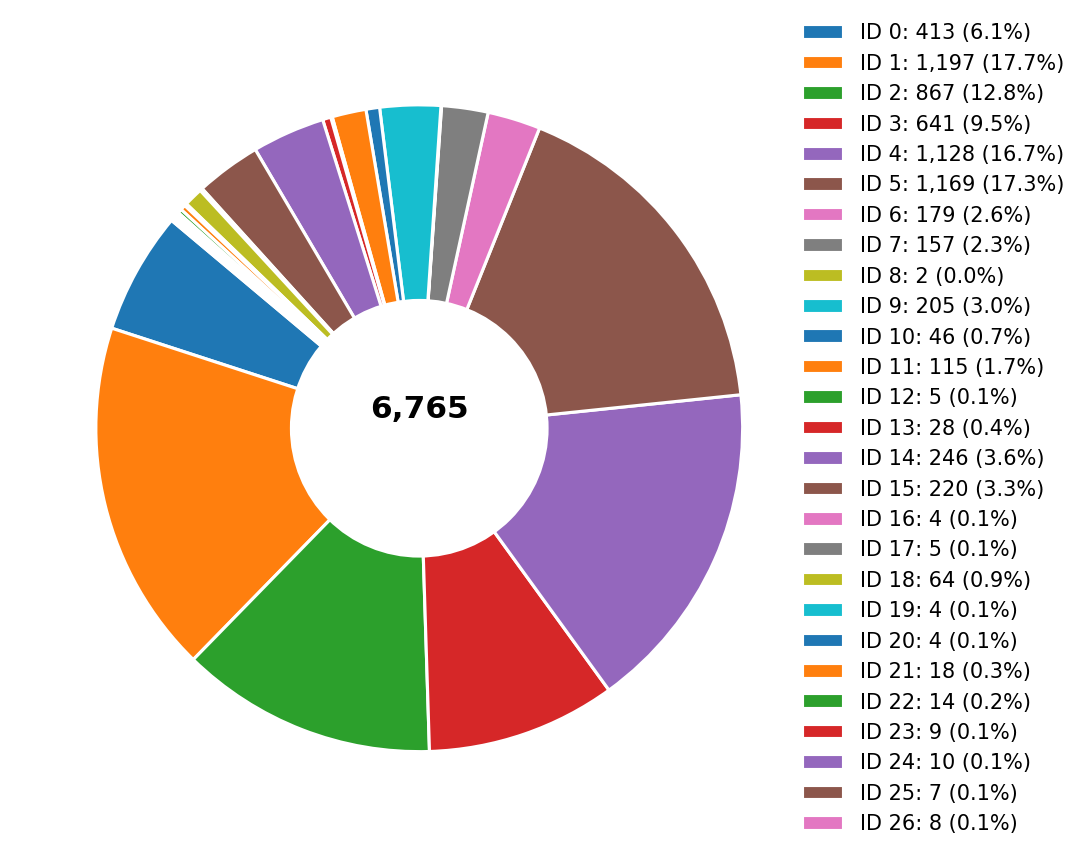
\includegraphics[width=0.7\linewidth]{Imagenes/communities_donut}
	\caption{}
	\label{fig:communitiesdonut}
\end{figure}

	\chapter{Herramienta de visualización de la red}
	
	Para poder explorar de forma interactiva la red de dependencias de Python se desarrolla una herramienta de visualización en tiempo real basada en un motor de físicas implementado íntegramente en Python. La herramienta, recogida en el script \texttt{visualizer.py}. Mediante esta aplicación se puede navegar a través de la red, inspeccionar diferentes métricas en función del nodo y ver como va variando la estructura de la red en función de las físicas escogidas con mejor rendimiento para redes de este tamaño que en Gephi.
	
	\section{Arquitectura general}

	
	El diseño de la herramienta se basa en las siguientes librerías principalmente:
	
	\begin{itemize}
		\item \texttt{igraph}: se utiliza para cargar el grafo desde el fichero \texttt{pypi\_multiseed\_10k.graphml} y del cálculo de la mayoría de métricas relacionadas con grafos vistas en clase.
		\item \texttt{vispy}: se utiliza como motor de renderizado interactivo que hace uso de OpenGL mediante aceleración por GPU y para capturar los inputs de teclado y ratón.
		\item \texttt{numpy}: se utiliza para la vectorización de todas las operaciones del motor de físicas y del cómputo de colores por nodo de manera eficiente.
	\end{itemize}
	
	La resolución del monitor se consulta en tiempo de ejecución a través de \texttt{glfw} antes de crear la ventana porque para que se vea adecuadamente la leyenda es necesario trabajar a pantalla completa. Se ha utilizado esta librería para el renderizado porque entre las distintas librerías dentro de \texttt{vispy} es la que mejor rendimiento ha dado en el equipo utilizado.
	
	\section{Cálculos preliminares}
	
	Para calcular una disposición inicial \enquote{razonable} de los nodos de manera eficiente, se emplea el algoritmo \textit{DrL} (Distributed Recursive Layout) integrado en la librería \texttt{igraph}. Aunque los reportes técnicos originales de este método ya no son de acceso público, su funcionamiento se encuentra documentado en el artículo correspondiente un algoritmo que lo mejora, la herramienta OpenOrd \cite{Martin2011OpenOrd}. En la figura \ref{fig:initial} se puede ver la distribución inicial que genera este algoritmo.
	\newline
	
	\begin{figure}[H]
		\centering
		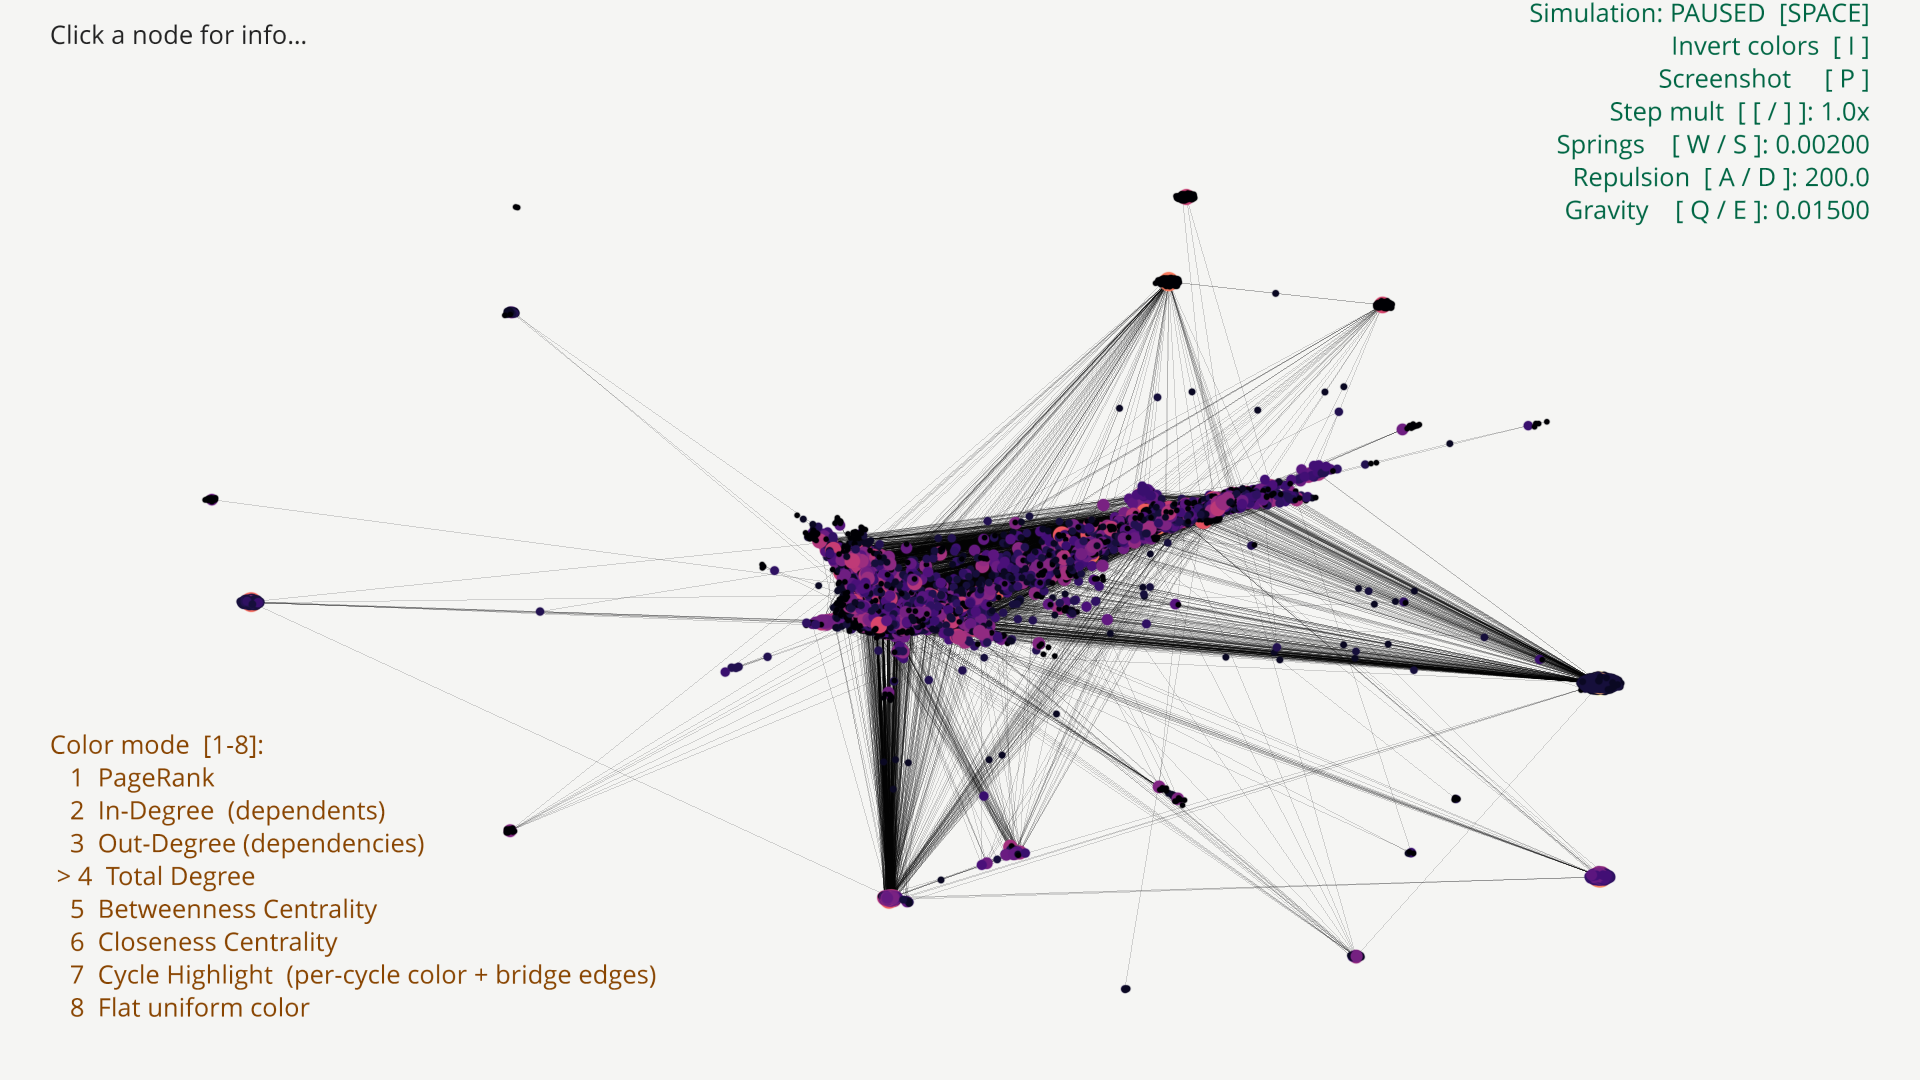
\includegraphics[width=1\linewidth]{Imagenes/Initial}
		\caption{Representación visual de la red tras aplicar el algoritmo DrL.}
		\label{fig:initial}
	\end{figure}
		
	El tamaño de cada nodo se determina mediante una normalización logarítmica del grado total para que los nodos de mayor tamaño sean más visibles, pero dejando un tamaño mínimo de 4 píxeles.
	
	\begin{equation}
		s_i = 21 \cdot \hat{G}_i + 4, \qquad \hat{G}_i = \frac{\log(1 + G_i^{\text{in}} + G_i^{\text{out}})}{\max_j \log(1 + G_j^{\text{in}} + G_j^{\text{out}})}
	\end{equation}
	donde \(s_i\) es el tamaño del nodo y \(G\) es el grado de entrada/salida de cada nodo.
	\newline
	
	En cuanto a las aristas para que los nodos se pudieran visualizar correctamente, estas se pintan \enquote{por debajo} en el lienzo por lo que las flechas de dirección no son fácilmente visibles. No obstante, como se puede alternar el esquema de colores para ver los grados de entrada y salida, al igual que hacer click en ellos, se puede saber fácilmente la direccionalidad de las flechas a nivel macroscópico. Además, para ver mejor la concentración de aristas cuando estas se superponen se reduce su transparencia por lo que se ve su color más marcado.
	
\section{Motor de físicas}
Para hacer la visualización más intuitiva del grafo en la herramienta se incorpora un motor de físicas basado en fuerzas que permite reorganizar el grafo en tiempo real. La simulación puede activarse y reanudarse con la tecla \texttt{ESPACIO}, y su velocidad se controla mediante un multiplicador ajustable. En cada fotograma (\texttt{on\_timer\_tick}), la fuerza neta $\mathbf{F}_i = \mathbf{F}_{\text{H}, i} + \mathbf{F}_{\text{g}, i} + \mathbf{F}_{\text{r}, i}$ aplicada sobre cada nodo $i$ con posición $\mathbf{p}_i$ (\texttt{pos}) se calcula como la suma de tres fuerzas principales:

\begin{itemize}
	\item \textbf{Fuerza de Hooke}: las aristas actúan como muelles que atraen los nodos conectados entre sí. Para un nodo $i$, la fuerza ejercida por el conjunto de sus nodos adyacentes $\mathcal{N}(i)$ se define como:
	$$\mathbf{F}_{\text{H}, i} = \sum_{j \in \mathcal{N}(i)} k_s (\mathbf{p}_j - \mathbf{p}_i)$$
	donde $k_s$ es \texttt{spring\_strength}. En la implementación, esto se vectoriza calculando la diferencia direccional (\texttt{p1 - p0}) y aplicando la fuerza simétricamente en ambos extremos de la arista.
	
	\item \textbf{Fuerza gravitatoria}: atrae a cada nodo hacia el origen de coordenadas $(0,0)$ con una intensidad proporcional a su grado total, manteniendo el grafo centrado y evitando la dispersión indefinida de los nodos más periféricos:
	$$\mathbf{F}_{\text{g}, i} = - k_g G_i \mathbf{p}_i$$
	donde $k_g$ es \texttt{gravity} y $G_i$ corresponde a su grado normalizado (\texttt{norm\_degrees\_2d}).
	
	\item \textbf{Fuerza repulsiva}: para que el programa no se congele al calcular la fuerza de repulsión de manera tradicional se calcula en cada frame las fuerzas de repulsión para un subconjunto $\mathcal{R}$ de tamaño $N_R = 300$ (\texttt{sample\_size}). De esta manera, aunque el calculo no es del todo exacto, se agilizan los cálculos y se asume que la distribución visual final no variaría demasiado en el equilibrio:
	$$\mathbf{F}_{\text{r}, i} = \sum_{j \in \mathcal{R}} k_r \frac{\mathbf{p}_i - \mathbf{p}_j}{\|\mathbf{p}_i - \mathbf{p}_j\|^2 + 1}$$
	donde $k_r$ es outward\_push. Se añade un \(+1\) en el denominador para evitar singularidades en el caso de que dos nodos estén superpuestos. Se utiliza esta formula de la fuerza para que los nodos tengan más alcance en la repulsión para reducir las aglomeraciones de nodos.
\end{itemize}

A partir de las fuerzas se calcula la velocidad en cada frame asumiendo un $\delta t =1$ y masa unitaria mediante integración numérica con un coeficiente de amortiguamiento $\mu$ caracterizado por la variable \texttt{"friction"} y limitada por una velocidad máxima (\texttt{"max\_speed"}).
$$\mathbf{v}_i^{(t+1)} = \left(\mathbf{v}_i^{(t)} + \mathbf{F}_{\text{total}, i}\right) \cdot \mu$$

Por último, se calculan las posiciones de manera análoga a las velocidad mediante integración discreta:
$$\mathbf{p}_i^{(t+1)} = \mathbf{p}_i^{(t)} + \mathbf{v}_i^{(t+1)}$$

De esta manera se puede ver como queda el resultado de aplicar el algoritmo tal y como se puede ver en la figura \ref{fig:full} en comparación con el estado inicial en la figura \ref{fig:initial}.

\begin{figure}
	\centering
	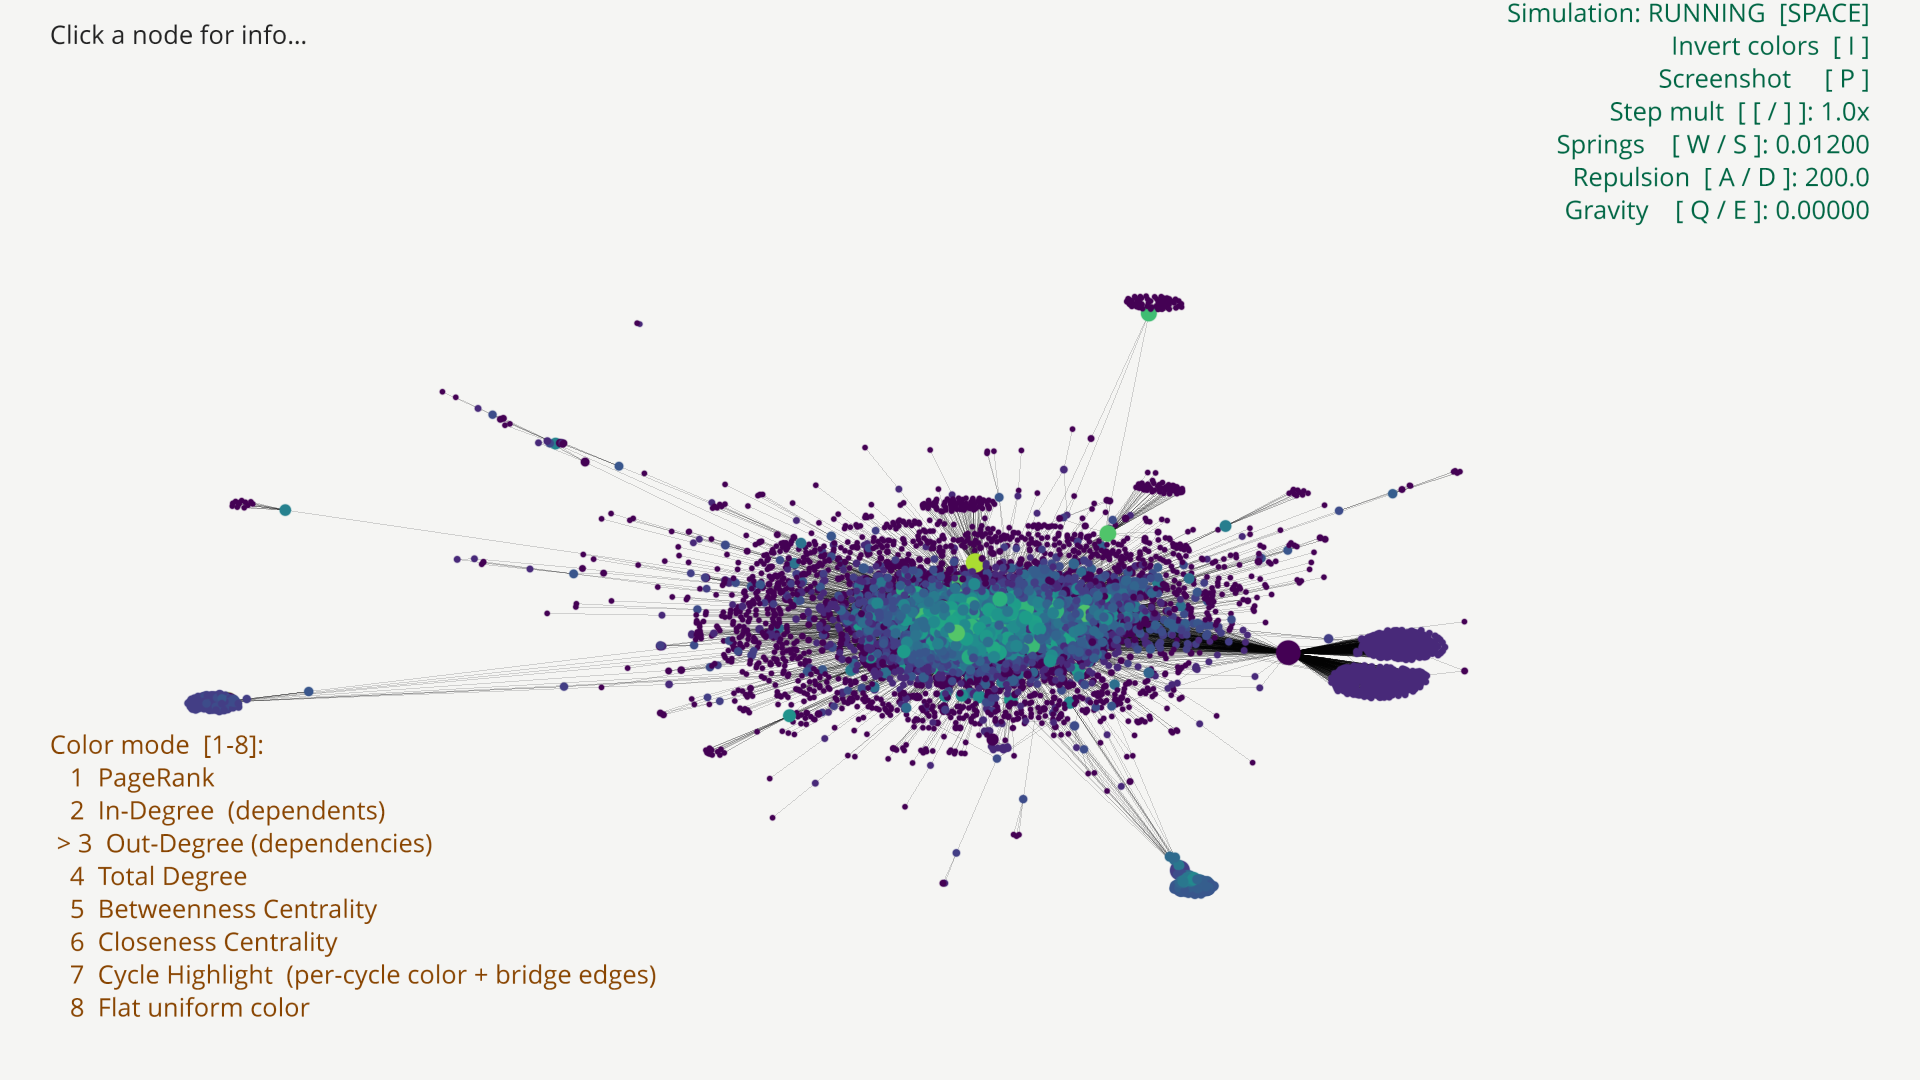
\includegraphics[width=1\linewidth]{Imagenes/Full}
	\caption{Representación de la red tras ejecutar el motor de físicas sobre la red hasta llegar al equilibrio.}
	\label{fig:full}
\end{figure}
	
	\section{Métricas y modos de color}
	Para agilizar la visualización de los datos en función de diferentes métricas o criterios se precalculan diferentes métricas y se almacenan normalizadas para representarse en diferentes escalas de color. Para alternar entre cada una de las visualizaciones se utilizan los números del 1 al 8. Los modos de color son los siguientes:
	
	\begin{enumerate}
		\item \textbf{PageRank}: con paleta \textit{plasma}.
		\item \textbf{Grado de entrada}: con paleta \textit{inferno}.
		\item \textbf{Grado de salida}: con paleta \textit{viridis}.
		\item \textbf{Grado total}: con paleta \textit{magma}.
		\item \textbf{Centralidad de intermediación} se utiliza una paleta con un degradado de negro a blanco pasando por rojo y amarillo.
		\item \textbf{Centralidad de cercanía} se utiliza una paleta con un degradado de azul oscuro a cian.
		\item \textbf{Destacado de ciclos}: se utiliza el método de la sección \ref{sec:ciclos}.
		\item \textbf{Comunidades (Louvain)}: cada nodo se colorea según la comunidad a la que pertenece.
	\end{enumerate}
	
	Las métricas de grado, PageRank, intermediación y cercania se normalizan en escala logarítmica (\(\log(1+x)\)).
	
	\section{Modo de visualización de ciclos}
	\label{sec:ciclos}
	
	El modo 7 está dedicado al análisis de las componentes fuertemente conexas (SCC) del grafo, es decir, los conjuntos de paquetes que forman dependencias circulares entre sí.
	\newline
	
	Al activar este modo, se calculan todas las SCC con más de un nodo. A cada ciclo se le asigna un tono único extraído de una paleta generada distribuyendo uniformemente los matices del espacio HSV:
	
	\begin{equation}
		H_k = \frac{k}{N_{\text{ciclos}}}, \quad k = 0, 1, \ldots, N_{\text{ciclos}} - 1
	\end{equation}
	
	Los nodos que no pertenecen a ningún ciclo se muestran en gris oscuro. Por otro lado, para añadir claridad se reestructura la coloración de las aristas:	
	\begin{itemize}
		\item \textbf{Aristas intraciclo}: conexiones entre nodos del mismo ciclo. Se colorean con el tono de su ciclo, con transparencia parcial, de forma que las aristas interpolan visualmente entre los colores de los nodos que unen.
		\item \textbf{Aristas interciclo}: conexiones que van de un ciclo a otro ciclo distinto. Se muestran en dorado semitransparente.
		\item \textbf{Aristas al resto}: las conexiones que involucran al menos un nodo fuera de cualquier ciclo se ocultan.
	\end{itemize}
	
	\section{Inversión de colores}
	
	La tecla \texttt{I} permite invertir la paleta de colores de toda la visualización. Se invierten los canales RGB de los nodos, el fondo pasa de negro a blanco y los colores del texto del se adaptan para mantener la legibilidad. Las aristas interciclo cambian del dorado al azul-violeta. Esta función resulta útil para capturas de pantalla.
	
	\section{Interacción}
	
	\subsection{Controles de teclado}
	
	La totalidad de los parámetros de la simulación y la visualización es ajustable sin interrumpir la ejecución. La Tabla \ref{tab:controles} resume los atajos disponibles.
	
	\begin{table}[H]
		\centering
		\caption{Atajos de teclado de la herramienta de visualización.}
		\label{tab:controles}
		\begin{tabular}{@{}ll@{}}
			\toprule
			\textbf{Tecla} & \textbf{Acción} \\
			\midrule
			\texttt{ESPACIO}       & Activar / pausar la simulación de físicas \\
			\texttt{1}--\texttt{8} & Cambiar el modo de coloración de nodos \\
			\texttt{I}             & Invertir la paleta de colores \\
			\texttt{W / S}         & Aumentar / reducir la rigidez de los muelles \\
			\texttt{A / D}         & Reducir / aumentar la fuerza de repulsión \\
			\texttt{Q / E}         & Aumentar / reducir la gravedad \\
			\texttt{[ / ]}         & Dividir / multiplicar por 10 el multiplicador\\
			\bottomrule
		\end{tabular}
	\end{table}
	
	\subsection{Inspección de nodos}
	
	Al hacer clic con el botón sobre un nodo se identifica el nodo más cercano al clic. Esto se realiza transformando las coordenadas de la pantalla al espacio del grafo mediante la inversa de la transformación de la cámara. Si la distancia al nodo más próximo es inferior a un umbral, se muestra en el texto superior izquierdo la siguiente información:
	
	\begin{itemize}
		\item Nombre del paquete.
		\item Grado de entrada y salida.
		\item Valor de la métrica activa para ese nodo.
		\item Identificador y tamaño del ciclo al que pertenece, o indicación de que el nodo no forma parte de ninguno.
		\item Identificador de la comunidad Louvain a la que pertenece el nodo.
	\end{itemize}
	\chapter{Conclusiones}
	
	% ── Bibliografía ─────────────────────────────────────────────────────────────
	\bibliography{referencias}   % n

\end{document}